\chapter{Maß  und Integrationstheorie}
\label{\detokenize{masstheorie/intro_masstheorie:masz-und-integrationstheorie}}\label{\detokenize{masstheorie/intro_masstheorie::doc}}
\par
Im ersten Semester haben wir bereits das \emph{Riemann Integral} zur Berechnung des Flächeninhalts zwischen einer Funktion \(f \colon [a,b] \rightarrow \R\) und der x Achse eingeführt (siehe Kapitel 7 in \cite{Bur20}).
Die grundlegende Idee hierbei war es die x Achse in (unterschiedlich große) Intervalle zu unterteilen und mittels dieser Zerlegung Rechtecke zwischen dem Graphen der Funktion und der x Achse zu konstruieren.
Durch das Produkt der Seitenlängen dieser Rechtecke lässt sich nämlich deren Flächeninhalt leicht berechnen und die Summe all dieser Flächeninhalte approximiert den wahren Flächeninhalt zwischen dem Graphen und \(f\) und der x Achse.
Dieses Vorgehen ist zur Erinnerung nochmal in Abbildung \hyperref[\detokenize{masstheorie/intro_masstheorie:fig-riemann-integral}]{Fig.\@ \ref{\detokenize{masstheorie/intro_masstheorie:fig-riemann-integral}}} illustriert.

\begin{figure}[htbp]
\centering


\noindent\includegraphics[width=\textwidth]{../\string_build/html/\string_images/ober\string_untersummen.png}
\caption{Illustration zweier Approximationen des Riemann Integrals einer Funktion durch den Flächeninhalt von Rechtecken. Die grünen und lila Rechtecke visualisieren die Unter  bzw. Obersummen bezüglich des in rot dargestellten Graphen der Funktion. Quelle: \href{https://de.wikipedia.org/wiki/Riemannsches\_Integral}{Wikipedia; Riemannsches Integral}.}\label{\detokenize{masstheorie/intro_masstheorie:fig-riemann-integral}}\end{figure}

\par
Da wir bisher nur die Integration von eindimensionalen Funktionen auf kompakten Intervallen kennengelernt haben, wollen wir in diesem Kapitel den Begriff des Integals auf mehrdimensionale Funktionen \(f \colon \R^n \rightarrow \R\) erweitern.
Das Riemann Integral lässt sich problemlos auf mehrdimensionalen Funktionen verallgemeinern, indem man das Integral nicht durch den Flächeninhalt von Rechtecken approximiert, sondern hierfür das \emph{Volumen von entsprechenden Quadern} \(Q \subset \R^n\) berechnet.
Es lässt sich insbesondere zeigen, dass jede stetige mehrdimensionale Funktion auf einem (nicht ausgeartetem) Quader Riemann integrierbar ist.

\par
Es hat sich jedoch in der Entwicklung der Mathematik herausgestellt, dass der Begriff des Riemann Integrals zu starke Forderungen an die zu Grunde liegenden Funktionen stellt und damit wichtige und interessante Funktionsklassen nicht integrierbar waren.
Als Beispiel hierfür seien \href{https://de.wikipedia.org/wiki/Fraktal}{fraktale Mengen und Funktionen} genannt, welche auch zur Modellierung von Prozessen in der Natur genutzt werden.

\par
Aus diesem Grund hat sich ein eigenes Feld innerhalb der modernen Analysis gebildet   die sogenannte \textbf{Maßtheorie}.
Es widmet sich hauptsächlich der Untersuchung von Maßen zur Berechnung von Längen, Flächen und Volumina in unterschiedlichen mathematischen Strukturen und Räumen.
Es wird klar, dass Integration und die Berechnung von Volumina eng miteinander zusammen hängen, denn ist \(A\subset\R^n\) eine (messbare) Teilmenge, dann ist ihr Maß gleich dem Integral ihrer charakteristischen Funktion, d.h.,
\begin{align*}
\int_{\R^n} \mathbb{1}_A(x)\,\mathrm{d}x.
\end{align*}
\par
In einem gewissen Sinn sind Maße ein \emph{fundamentaleres Konzept} als das der Integration, da sich jede Integration auf die Berechnung von Maßen stützt.

\par
Eins der berühmtesten Beispiele zur Motivation der Maßtheorie ist im Folgenden erklärt.
\begin{example}{(Dirichlet Funktion)}{masstheorie/intro_masstheorie:ex:dirichletFunktion}



\par
Wir betrachten das kompakte Intervall \([0,1] \subset \R\) und definieren hierauf die sogenannte \textbf{Dirichlet Funktion} \(\mathbb{1}_\Q \colon [0,1] \rightarrow \{0,1\}\) mit
\begin{align*}
\mathbb{1}_\Q(x) := \begin{cases} 1, \ \text{ falls } x \in \Q, \\ 0, \ \text{ sonst }.\end{cases}
\end{align*}
\par
Diese Abbildung kann als \emph{charakteristische Funktion} der rationalen Zahlen \(\Q\) aufgefasst werden.
Man sieht leicht ein, dass diese Funktion \textbf{nicht Riemann integrierbar} ist, da alle Untersummen stets \(0\) und alle Obersummen stets \(1\) sind.
\end{example}

\par
Um eine Funktion wie die Dirichlet Funktion in \cref{masstheorie/intro_masstheorie:ex:dirichletFunktion} zu integrieren sieht man zunächst ein, dass die rationalen Zahlen \(\Q\) in den reellen Zahlen \(\R\) als abzählbare Menge eine sogenannte \emph{Nullmenge} im Sinne der Maßtheorie repräsentieren.
Wir werden im Laufe der Vorlesung die nötigen Werkzeuge der Maßtheorie einführen um diesen Umstand zu verstehen und einen verallgemeinerten Begriff des Integrals definieren, der diese Nullmenge berücksichtigt   das \textbf{Lebesgue Integral}.
Dieses Integral ist eine echte Verallgemeinerung des Riemann Integrals und wir werden einsehen, dass die Menge der Lebesgue integrierbaren Funktionen eine Obermenge der Menge der Riemann integrierbaren Funktionen ist.
Außerdem verhält sich das Lebesgue Integral bei Grenzwertbildungen einfacher als das Riemann Integral.


\section{Maßtheorie}
\label{\detokenize{masstheorie/masstheorie:masztheorie}}\label{\detokenize{masstheorie/masstheorie::doc}}
\par
Wir wollen in diesem Kapitel formal die Maßtheorie einführen, die es uns erlaubt zu entscheiden welche Mengen messbar sind und wie sich das Volumen von Mengen in topologischen Räumen bestimmen lässt.
Die hier beschriebenen Werkzeuge werden uns im nächsten Kapitel bei der Einführung des \emph{Lebesgue Integrals} als Verallgemeinerung des Riemann Integrals sehr dienlich sein.

\par
Intuitiv ordnet ein \href{https://de.wikipedia.org/wiki/Ma\%c3\%9f\_(Mathematik)}{\textbf{Maß}} \(\mu\), welches auf einer Menge \(\Omega\) definiert ist, wie z.B. dem \(\R^n\), allen geeigneten Teilmengen \(A\subseteq \Omega\) nichtnegative reelle Zahlen zu, d.h.
\begin{align*}
\mu(A)\in[0,\infty] := [0,\infty)\cup\{\infty\}.
\end{align*}
\par
Hierbei soll das Maß \(\mu\) natürlich mit dem Volumen der Teilmenge \(A\) zusammenhängen.
Man beachte, dass wir auch explizit unendliche Maße zulassen, z.B., falls die Menge \(\Omega\) schon der gesamte \(\R^n\) ist.

\par
Bevor wir den Begriff des Maßes formal definieren können und dessen Eigenschaften näher diskutieren, müssen wir jedoch noch mehr Verständnis für die zu Grunde liegenden Mengen und Mengensystem entwickeln.


\subsection{\protect\(\sigma\protect\) Algebren und Maße}
\label{\detokenize{masstheorie/masstheorie:sigma-algebren-und-masze}}
\par
Wir betrachten im Folgenden immer eine zu Grunde liegende Menge \(\Omega\).
Diese kann endlich, abzählbar unendlich oder auch überabzählbar unendlich sein.
Wir betrachten nun die \textbf{Potenzmenge} \(2^\Omega \equiv\mathcal{P}(\Omega)\) von \(\Omega\), welche die Menge aller möglichen Teilmengen von \(\Omega\) bildet.
Solche Mengen von Mengen nennen wir häufig \emph{Mengensysteme}.
In der Maßtheorie sind bestimmte Mengensysteme \(\mathcal{A} \subseteq \mathcal{P}(\Omega)\) zentral, nämlich die der \emph{meßbaren} Teilmengen von \(\Omega\).
Das sind die Mengen, denen ein Maß zugeordnet werden kann, also eine nichtnegative Zahl oder unendlich.

\par
Zunächst müssen wir klären, welche Teilmengen der Grundmenge \(\Omega\) überhaupt messbar sein sollen.
Am Einfachsten wäre es natürlich, alle möglichen Teilmengen messen zu können, also als Mengensystem \(\mathcal{A} = \mathcal{P}(M)\) zu betrachten.
Wir wir sehen werden ist dies leider nicht immer möglich, denn es existieren \emph{nichtmessbare Mengen}.
Es hat sich herausgestellt, dass es vernünftig ist zu fordern, dass das Mengensystem \(\mathcal{A}\) eine sogenannte \(\sigma\) Algebra ist, welche wir in der folgenden Definition einführen werden.
\begin{definition}{(\protect\(\sigma\protect\) Algebra und Messraum)}{masstheorie/masstheorie:def:sigmaalgebra}



\par
Ein Mengensystem \(\mathcal{A} \subseteq \mathcal{P}(\Omega)\) heißt \textbf{\(\sigma\) Algebra (von \(\Omega\))}, wenn die folgenden Eigenschaften erfüllt sind
\begin{enumerate}

\item {} 
\par
\(\Omega\in \mathcal{A}\)

\item {} 
\par
\(A\in \mathcal{A} \quad \Rightarrow \quad A^c:=\Omega \setminus A\in \mathcal{A}\)

\item {} 
\par
\((A_n)_{n\in\N} \in \mathcal{A} \quad \Rightarrow \quad \bigcup_{n\in \N} A_n\in \mathcal{A}\).

\end{enumerate}

\par
Für eine \(\sigma\) Algebra \(\mathcal{A} \subseteq \mathcal{P}(\Omega)\) von \(\Omega\) nennen wir das Paar (\(\Omega,\mathcal{A}\)) \textbf{Messraum} und die Mengen des Mengensystems \(\mathcal{A}\) heißen \textbf{messbar}.
\end{definition}

\par
Das Symbol \(\sigma\) erinnert uns an den Begriff der Summe, insbesondere wegen der dritten Eigenschaft in \cref{masstheorie/masstheorie:def:sigmaalgebra}  also der Abgeschlossenheit unter abzählbarer Vereinigung von Teilmengen.
Aus diesen drei Eigenschaften lässt sich auch direkt zeigen, dass \(\sigma\) Algebren ebenfalls unter \emph{abzählbaren Schnitten} abgeschlossen sind, wie das folgende Lemma zeigt.
\begin{lemma}{(Abgeschlossenheit unter abzählbaren Schnitten)}{masstheorie/masstheorie:lemma-1}



\par
Es sei (\(\Omega,\mathcal{A}\)) ein Messraum und es sei \((A_n)n_\N\) eine Familie von Elementen der \(\sigma\) Algebra \(\mathcal{A}\) mit \(A_n \in \mathcal{A}\) für \(n \in \N\).
Dann sind abzählbare Schnitte dieser Mengen auch Elemente der \(\sigma\) Algebra \(\mathcal{A}\), d.h.,
\begin{align*}
\bigcap_{n \in \N} A_n \in \mathcal{A}.
\end{align*}\end{lemma}

\begin{proof}
 In der Hausaufgabe zu zeigen.
\end{proof}

\par
Aus der \cref{masstheorie/masstheorie:def:sigmaalgebra} kann man sich leicht zwei Spezialfälle von \(\sigma\) Algebren überlegen.
Es wird klar, dass das Mengensystem \(\{\emptyset, \Omega\}\) die kleinstmögliche \(\sigma\) Algebra bildet, wohingegen die Potenzmenge \(\mathcal{P}(\Omega)\) die größtmögliche \(\sigma\) Algebra darstellt.

\par
Basierend auf dem Begriff einer \(\sigma\) Algebra und eines Messraums können wir nun formal einführen, was wir mathematisch unter einem Maß verstehen.
\begin{definition}{(Maß und Maßraum)}{masstheorie/masstheorie:def:mass}



\par
Sei \((\Omega, \mathcal{A})\) ein Messraum.
Wir nennen eine Abbildung \(\mu: \mathcal{A}\to [0, \infty]\) \textbf{Maß}, wenn die folgenden beiden Eigenschaften erfüllt sind.
\begin{enumerate}

\item {} 
\par
Die leere Menge hat das Maß Null, d.h., \(\mu(\emptyset) = 0\),

\item {} 
\par
Für eine Familie von disjunkten Mengen \((A_n)_{n\in\N}\) der \(\sigma\) Algebra \(\mathcal{A}\) mit \(A_i \cap A_j = \emptyset\) für \(i \neq j\) gilt die sogenannte abzählbare oder \(\sigma\) \textbf{Additivität}, d.h.,

\end{enumerate}
\begin{align*}
\mu\left( \bigcup_{n\in\N}A_n \right) = \sum_{n\in\N}\mu (A_n).
\end{align*}
\par
Wir nennen das Maß \(\mu\) \textbf{endlich}, wenn \(\mu(\Omega)<\infty\).
Das Tripel aus zu Grunde liegender Menge, \(\sigma\) Algebra und Maß \((\Omega, \mathcal{A}, \mu)\) wird als \textbf{Maßraum} bezeichnet.
\end{definition}
\begin{remark}{}{masstheorie/masstheorie:rem:wahrscheinlichkeitsmass}



\par
Maße spielen insbesondere in der \emph{Wahrscheinlichkeitstheorie} eine zentrale Rolle.
Hier werden Sie die benötigt um die Wahrscheinlichkeit von Ereignismengen anzugeben.
Dabei wird nicht nur gefordert, dass das Maß \(\mu\) endlich sein muss, sondern dass sogar \(\mu(\Omega)=1\) gilt, damit es sich um ein \textbf{Wahrscheinlichkeitsmaß} handelt.
Diese finden vor allem in der Quantenmechanik Anwendung.
\end{remark}

\par
Aus den beiden grundlegenden Eigenschaften eines Maßes lassen sich weitere nützliche Eigenschaften herleiten, wie das folgende Lemma beschreibt.
\begin{lemma}{(Eigenschaften von Maßen)}{masstheorie/masstheorie:lemma-4}



\par
Sei \((\Omega, \mathcal{A}, \mu)\) ein Maßraum.
Dann gelten die folgenden Eigenschaften für das Maß \(\mu \colon \mathcal{A} \rightarrow [0,\infty]\).

\par
1. Für \(A,B \in \mathcal{A}\) mit \(B \subset A\) und \(\mu(B) < \infty\) gilt:
\begin{align*}
\mu(A \setminus B) = \mu(A) - \mu(B) \qquad \text{(Subtraktivität)}
\end{align*}
\par
2. Für \(A,B \in \mathcal{A}\) mit \(B \subset A\) gilt:
\begin{align*}
\mu(B) \leq \mu(A) \qquad \text{(Monotonie)}
\end{align*}
\par
3. Für \(A,B \in \mathcal{A}\) gilt stets:
\begin{align*}
\mu(A \cup B) = \mu(A) + \mu(B) - \mu(A \cap B).
\end{align*}\end{lemma}

\begin{proof}
 In der Hausaufgabe zu zeigen.
\end{proof}

\par
Im Folgenden wollen wir ein paar Beispiele von geläufigen Maßen diskutieren.
\begin{example}{(Maße)}{masstheorie/masstheorie:example-5}



\par
Wichtige Maße in der Mathematik und Physik sind beispielsweise die folgenden.

\par
1. Das \href{https://de.wikipedia.org/wiki/Z\%c3\%a4hlma\%c3\%9f\_(Ma\%c3\%9ftheorie)}{\textbf{Zählmaß}} \(m\) auf einer \emph{endlichen} Menge \(M\), mit
\begin{align*}
m(A):=|A|\qquad (A\subseteq M).
\end{align*}
\par
Hier sind insbesondere alle Teilmengen messbar, d.h., \((M, \mathcal{P}(M), m)\) bildet einen Maßraum.

\par
2. Das \textbf{Lebesgue–Maß} \(\lambda^n\) auf dem \(\R^n\), das wir bald kennen lernen, zeichnet sich dadurch aus, dass es einer verschobenen Menge das gleiche Volumen zuordnet wie einer unverschobenen.
Es besitzt also die nützliche Eigenschaft \emph{translations } und \emph{rotationsinvariant} zu sein.
Dies gilt ebenfalls für Spiegelungen.
Außerdem ordnet das Lebesgue Maß dem Einheitswürfel \([0,1]^n\) das Maß \(1\) zu, was unserer Intuition entspricht.
Andererseits stellt sich heraus, dass das Lebesgue Maß nicht auf der gesamten Potenzmenge \(\mathcal{P}(\R^n)\) definiert werden kann.

\par
3. Das \href{https://de.wikipedia.org/wiki/Diracma\%c3\%9f}{\textbf{Dirac Maß}} \(\delta_x\) ist im Punkt \(x \in \R^n\) konzentriert, und für jede Teilmenge \(A\subset\R^n\) gilt
\begin{align*}
\delta_x(A) \equiv \int_A\delta_x := \begin{cases} 1, &  \text{ falls } x \in A,\\ 0, & \text{ sonst}. \end{cases}
\end{align*}
\par
Dieses Maß ist im Gegensatz zum Lebesgue Maß nicht translationsinvariant, da es explizit von der Lage des Punkts \(x\in\R^n\) abhängt.
Es wird beispielsweise in der Elektrodynamik benutzt, um eine in \(x\) lokalisierte, punktförmige Ladung zu beschreiben.

\par
4. Häufig möchte man die Länge einer \emph{Kurve} oder allgemeiner den Flächeninhalt einer \(d\) dimensionalen Fläche im \(\R^n\) messen.
Auch das dafür benutzte Maß \(\mu_d\) ist translations  und rotationsinvariant, es ordnet aber der \(d\) dimensionalen Einheitsfläche \([0,1]^d\times\{0\} \subset\R^d\times\R^{n-d}=\R^n\) das Maß \(1\) zu.
Entsprechend hat aber für \(d<n\) der Einheitswürfel das Maß \(\mu_d([0,1]^n)=\infty\).

\par
5. Man kann sogar sogenannte \href{https://de.wikipedia.org/wiki/Hausdorff-Ma\%c3\%9f}{\textbf{Hausdorff Maße}} \(\mu_d\) konstruieren, die Mengen beliebiger fraktaler Dimension \(d\in[0,n]\) messen.
Genau genommen \emph{definiert} man hierbei die Dimension der Menge \(A\subset \R^n\) durch \(d(A):=\inf\{d'>0\mid \mu_{d'}(A)=0\}.\)

\par
6. Im Zusammenhang mit dem sogenannten Feynmanschen \href{https://de.wikipedia.org/wiki/Pfadintegral}{\textbf{Pfadintegral}} der Quantenmechanik wird auf dem unendlich dimensionalen Raum \(\Omega\) der Weg zwischen zwei Punkten des Konfigurationsraumes \(\R^d\) ein \emph{Wahrscheinlichkeitsmaß} (siehe \cref{masstheorie/masstheorie:rem:wahrscheinlichkeitsmass}  definiert.
Dabei erhalten Pfade, die in der Nähe von Lösungskurven der DGL der Klassischen Mechanik sind, ein größeres Gewicht als beliebige Pfade.
\end{example}

\par
Eine sehr nützliche Eigenschaft von gewissen Maßen auf topologischen Räumen ist die der Regularität, welche wir im Folgenden definieren wollen.
\begin{definition}{(Regularität von Maßen)}{masstheorie/masstheorie:def:regularitaet}



\par
Es sei \((\Omega, \tau)\) ein topologischer Raum und \((\Omega, \mathcal{A}, \mu)\) ein entsprechender Maßraum auf \(\Omega\), so dass gilt \(\tau \subset \mathcal{A}\).
Dann können wir die Regulariät des Maßes \(\mu\) wie folgt definieren.
\begin{enumerate}

\item {} 
\par
Wir nennen das Maß \(\mu\) von \textbf{außen regulär}, wenn zu jeder messbaren Menge \(A \in \mathcal{A}\) und jedem \(\epsilon > 0\) eine offene Obermenge \(U \in \tau\) existiert mit \(A \subset U\), so dass für das Maß \(\mu(U\setminus A) < \epsilon\) gilt.

\item {} 
\par
Wir nennen das Maß \(\mu\) von \textbf{innen regulär}, wenn zu jeder messbaren Menge \(A \in \mathcal{A}\) und jedem \(\epsilon > 0\) eine abgeschlossene Teilmenge \(F \subset A\) gibt, so dass für das Maß \(\mu(A\setminus F) < \epsilon\) gilt.

\end{enumerate}
\end{definition}

\par
Hier noch eine Abbildung oder ein Beispiel zu Regularität?


\subsection{Borel Maße}
\label{\detokenize{masstheorie/masstheorie:borel-masze}}
\par
Da es viele unterschiedliche Möglichkeiten gibt eine Menge in Teilmengen zu unterteilen wünscht man sich eine möglichst kanonische Wahl einer \(\sigma\) Algebra.
Es stellt sich heraus, dass die sogenannte Borel \(\sigma\) Algebra eine gute Wahl auf beliebigen topologischen Räumen definiert.

\begin{emphBox}{}{}

\par
\href{https://de.wikipedia.org/wiki/\%C3\%89mile\_Borel}{Émile Borel} (geboren am 7. Januar 1871 in Saint Affrique; gestorben am 3. Februar 1956 in Paris) war ein französischer Mathematiker und Politiker.
\end{emphBox}
\begin{definition}{(Borel \protect\(\sigma\protect\) Algebra)}{masstheorie/masstheorie:definition-7}



\par
Die \textbf{Borel \(\sigma\) Algebra} auf einem topologischen Raum \((\Omega, \tau)\) ist die kleinste \(\sigma\) Algebra auf der Menge \(\Omega\), die die Topologie \(\tau\) enthält, d.h.
\begin{align*}
\B(\Omega) := \bigcap_{\substack{\mathcal{A} \text{ ist $\sigma$-Algebra}\\ \tau \subset \mathcal{A}}} \mathcal{A}
\end{align*}
\par
Man nennt die Borel \(\sigma\) Algebra auch \textbf{die von \(\tau\) erzeugte \(\sigma\) Algebra}.
\end{definition}

\par
Die folgende Bemerkung beschreibt die Borel \(\sigma\) Algebra, wenn als zu Grunde liegende Menge die reellen Zahlen \(\R\) gewählt werden, wie es häufig in Anwendungen der Fall ist.
\begin{remark}{(Borelsche \protect\(\sigma\protect\) Algebra von \protect\(\R\protect\))}{masstheorie/masstheorie:remark-8}



\par
Wir untersuchen den topologischen Raum \((\R, \tau)\), wobei die Topologie \(\tau\) gerade alle offenen Intervalle \((a,b) \subset \R\) mit rationalen Punkten \(a,b \in \Q\) enthält.
Da dies die kanonische Topologie für die reellen Zahlen bildet sprcht man bei der von ihr erzeugten Borel \(\sigma\) Algebra als \emph{die} Borelsche \(\sigma\) Algebra.

\par
Sie enthält alle wichtigen Teilmengen von \(\R\), nämlich:
\begin{itemize}
\item {} 
\par
alle \emph{offenen, abgeschlossenen} und \emph{kompakten} Mengen

\item {} 
\par
alle \emph{Intervalle} der Form \((a,b), [a,b], (a,b], [a,b]\) für \(a,b \in \R\), sowie alle Intervalle der Form \((-\infty, b), (-\infty, b]\) und \((a, \infty), [a,\infty)\)

\item {} 
\par
alle \emph{Punktmengen} der Form \(\{a\}\) für \(a \in \R\)

\item {} 
\par
alle \emph{endlichen} Teilmengen von \(\R\)

\item {} 
\par
alle \emph{unendlich abzählbaren} Teilmengen von \(\R\)

\end{itemize}

\par
Wir bemerken, dass die Borelsche \(\sigma\) Algebra von \(\R\) \textbf{nicht} alle Teilmengen von \(\R\) enthält.
Es lässt sich sogar zeigen, dass die borelsche \(\sigma\) Algebra von \(\R\) gleichmächtig zu \(\R\) ist, während die Potenzmenge \(\mathcal{P}(\R)\) von \(\R\) eine echt größere Mächtigkeit als \(\R\) besitzt.
\end{remark}

\par
Für spezielle topologische Räume lässt sich eine wichtige Eigenschaft von Maßen über die Borel \(\sigma\) Algebra definieren.
\begin{definition}{(Lokale Endlichkeit von Maßen)}{masstheorie/masstheorie:definition-9}



\par
Sei \((\Omega, \tau)\) ein Haussdorf Raum (siehe \cref{manifolds/manifolds_prelim:def:hausdorffraum}  und sei \(\B(\Omega) = \sigma(\tau)\) die Borel \(\sigma\) Algebra, die durch \(\tau\) erzeugt wird.
Wir nennen ein Maß \(\sigma \colon \B(\Omega) \rightarrow [0, \infty]\) \textbf{lokal endlich}, falls jeder Punkt \(x \in \Omega\) eine lokale Umgebung mit endlichem Maß besitzt.
\end{definition}

\par
Die lokale Endlichkeit ist essentiell bei der Untersuchung von Maßen auf topologischen Räumen, weil sie für jeden Punkt die Existenz einer Umgebung mit endlichem Maß garantiert.
Wie wir später sehen werden ist das Lebesgue Maß auf dem Raum \(\R^n\) lokal endlich.

\par
Basierend auf der oben definierten Borel \(\sigma\) Algebra lässt sich nun das sogenannte Borel Maß einführen.
\begin{definition}{(Borel Maß)}{masstheorie/masstheorie:definition-10}



\par
Ein lokal endliches Maß \(\sigma \colon \B(\Omega) \rightarrow [0, \infty]\) auf der Borelschen \(\sigma\) Algebra eines Hausdorff Raums \((\Omega,\tau)\) heißt \textbf{Borel Maß}.
\end{definition}


\subsection{Das Lebesgue Maß}
\label{\detokenize{masstheorie/masstheorie:das-lebesgue-masz}}
\begin{emphBox}{Henri Lebesgue}{}

\par
\href{https://en.wikipedia.org/wiki/Henri\_Lebesgue}{Henri Léon Lebesgue} (Geboren 28. Juni 1875 in Beauvais; Gestorben 26. Juli 1941 in Paris) war ein französischer Mathematiker.
\end{emphBox}

\par
Bei der Einführung des Riemann Integrals verwendet man Intervalle zur Unterteilung des Definitionsbereichs.
Diese Partitionierung einer Menge lässt sich im \(\R^n\) auf mehrdimensionale Quader verallgemeinern. Für \(a = (a_1,\ldots,a_n) \in \R^n\) und \(b = (b_1,\ldots,b_n) \in \R^n\) verwenden wir hierbei die Anordnungsrelation
\begin{align*}
a < b \qquad \Leftrightarrow \qquad a_i < b_i \quad i=1,\ldots,n
\end{align*}
\par
und analog für \(a \leq b, a > b\) und \(a \geq b\).
\begin{definition}{(Mehrdimensionale Quader)}{masstheorie/masstheorie:def:quader}



\par
und darüber im Folgenden \textbf{offene, halboffene} und \textbf{abgeschlossene Quader} im \(\R^n\) respektive beschreiben durch
\begin{align*}
(a,b) &= \lbrace x \in \R^n : a < x < b \rbrace,\\
(a,b] &= \lbrace x \in \R^n : a < x \leq b \rbrace,\\
[a,b] &= \lbrace x \in \R^n : a \leq x \leq b \rbrace.
\end{align*}
\par
Das \textbf{Volumen} bzw. der Lebesgue Inhalt eines halboffenen Quaders \(Q := (a,b] \subset \R^n\) definieren wir über
\begin{align*}
\lambda^n(Q) := \prod_{i=1}^n (b_i - a_i).
\end{align*}\end{definition}

\par
Wir wollen im Folgenden das Teilmengensystem \(\mathcal{R}_{\text{Q}}\subset\ 2^{\R^n}\) aller halboffenen Quader betrachten,
\begin{align*}
\mathcal{R}_{\text{Q}} := \left\{ \bigsqcup_{i=1,\ldots,k} Q_i \colon Q_i \text{ ist halboffener Quader im } \R^n \right\}.
\end{align*}
\par
Wir fordern hierbei nicht, dass nur disjunkte Quader vereinigt werden dürfen. Jedoch kann man direkt herleiten, dass man jede Vereinigung von Quadern in eine disjunkte Umschreiben kann. Seien dazu \(Q_1,\ldots,Q_k\subset\R^n\) halboffene Quader, wir erkennen, dass der Rand eines Quaders \(Q_i=(a^i,b^i]\) genau \(2n\) Hyperebenen der Form
\begin{align*}
x_j = a^i_j\\
x_j = b^i_j
\end{align*}
\par
für \(j=1,\ldots,n\) aufspannt. Weiterhin, können wir einen anderen Quader \(Q_m=(a^k,b^k)\) mit einer Hyperebene \(x_l=c\in\R\) zerteilen, im Falle \(a^k_l < c < b^k_l\), indem wir zwei neue Quader definieren mit
\begin{align*}
\alpha^m&:=(a^m_1,\ldots,c,\ldots,a^m_n)\\
\beta^m&:=(b^m_1,\ldots,c,\ldots,b^m_n)\\
Q_m^1&=(a^m,\beta^m]\\
Q_m^2&=(\alpha^m,b^m].
\end{align*}
\par
Iterativ gehen wir folgendermaßen vor:
\begin{enumerate}

\item {} 
\par
Betrachten den ersten Quader \(Q_1\), zerteilen alle Quader \(Q_i\) an allen seinen Hyperebenen und erhalte so neue Quader \(W^1_j\).

\item {} 
\par
Im \(i+1\)ten Schritt betrachte die Hyperebenen des Quaders \(Q_{i+1}\) und zerteile damit alle Quader \(W^i_j\) aus dem vorherigen Schritt und erhalte damit neue Quader \(W^{i+1}_j\).

\end{enumerate}

\par
Führen wir diesen Prozess bis \(i=k\) durch, so erhalten wir folgendes Resultat, welches in {fig:disrect broken reference} visualisiert ist.

\begin{figure}[htbp]
\centering


\noindent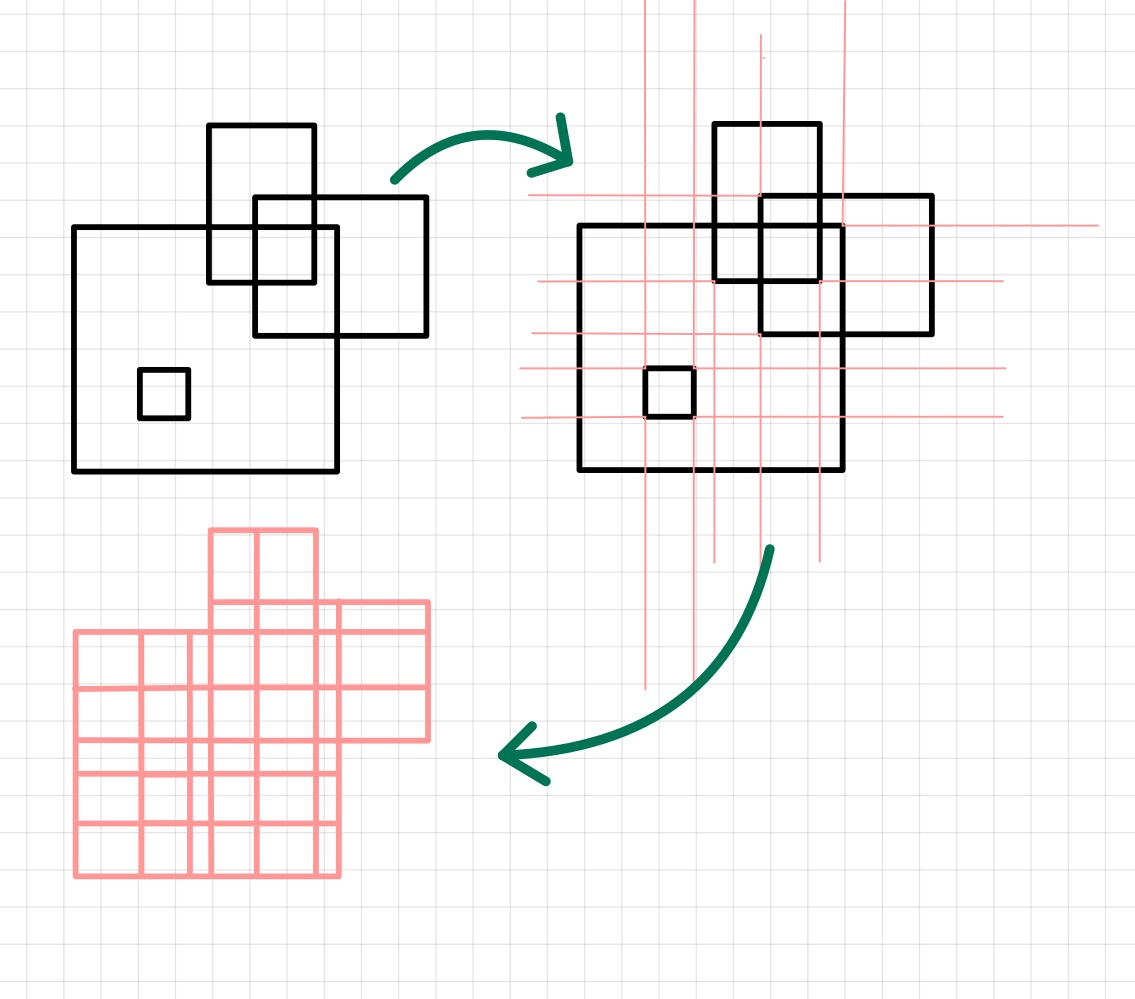
\includegraphics[width=\textwidth]{../\string_build/html/\string_images/DisRect.jpg}
\caption{Nicht disjunkte Quader werden in System disjunkter Quader überführt. Man erkennt insbesondere, dass die Vereinigung gleich bleibt und, dass sich jeder einzelne ursprüngliche Quader, aus den neuen Quadern zusammensetzbar ist.}\label{\detokenize{masstheorie/masstheorie:fig-disrect}}\end{figure}
\begin{lemma}{}{masstheorie/masstheorie:lem:disRect}



\par
Es seien \(Q_1,\ldots,Q_k\subset\R^d\) halboffene Quader, dann existieren paarweise disjunkte halboffene Quader \(W_1,\ldots, W_M\) mit Indexmengen \(J_i\subset\{1,\ldots,M\}\), s.d.
\begin{align*}
\bigcup_{i=1}^k Q_i = \bigcup_{j=^1}^M W_j
\end{align*}
\par
und für jedes \(i\in\{1,\ldots,n\}\) gilt
\begin{align*}
\bigcup_{j\in J_i} W_j = Q_i.
\end{align*}\end{lemma}

\par
Das System der halboffenen Quadern bildet eine besondere mathematische Struktur, einen sogenannten Mengen Ring.
\begin{definition}{(Ring)}{masstheorie/masstheorie:def:ring}



\par
Ein Mengensystem \(\mathcal{R} \subset 2^{\Omega}\) heißt \textbf{Mengen Ring} (im maßtheoretischen Sinne) auf einer Menge \(\Omega\), falls die folgenden Eigenschaften erfüllt sind:
\begin{enumerate}

\item {} 
\par
\(\emptyset \in \mathcal{R}\)

\item {} 
\par
\(A,B \in \mathcal{R} \Rightarrow (A \setminus B) \in \mathcal{R}\)

\item {} 
\par
\(A,B \in \mathcal{R} \Rightarrow (A \cup B) \in \mathcal{R}\)

\end{enumerate}
\end{definition}
\begin{lemma}{(Der von halboffenen Quadern erzeugte Ring)}{masstheorie/masstheorie:lemma-14}



\par
Das System der halboffenen Quadern \(\mathcal{R}_{\text{Q}}\) bildet einen Mengenring.
\end{lemma}

\begin{proof}
 Um zu zeigen, dass es sich bei dem Mengensystem \(\mathcal{R}_{\text{Q}}\) um einen Ring handelt müssen wir die Eigenschaften aus \cref{masstheorie/masstheorie:def:ring} nachweisen.

\par
1. Für einen beliebigen Punkt \(a \in \R^n\) gilt \(\emptyset = (a,a] \in \mathcal{R}_{\text{Q}}\).

\par
2. Als nächstes müssen wir zeigen, dass für zwei Mengen \(A,B \in \mathcal{R}_{\text{Q}}\) gilt, dass auch die Mengendifferenz in \(\mathcal{R}_{\text{Q}}\) enthalten ist, d.h., dass gilt \((A \setminus B) \in \mathcal{R}_{\text{Q}}\). Nach \{prf:ref\}``disRect` existieren paarweise disjunkte halboffene Quader \(S_j\), \(j=1,\ldots,n\), und Indexmengen \(I_A,I_B\subset\{1,\ldots,n\}\), s.d.,
\begin{align*}
A = \bigcup_{j\in I_A} S_j\\
B = \bigcup_{j\in I_B} S_j.
\end{align*}
\par
Somit gilt dann
\begin{align*}
A\setminus B &= \left(\bigcup_{j\in I_A} S_j\right) \setminus \left(\bigcup_{j\in I_B} S_j\right)\\ 
&= \bigcup_{j\in I_A\setminus I_B} S_j
\end{align*}
\par
was wieder eine Vereinigung von halboffenen Quadern ist und deshalb gilt \(A\setminus B\in \mathcal{R}_{\text{Q}}\).

\par
3. Zuletzt erkennen wir für zwei Mengen \(A,B \in \mathcal{R}_{\text{Q}}\), dass mit der Zerlegung aus 2. gilt
\begin{align*}
A\cup B = \bigcup_{j=1}^n S_j
\end{align*}
\par
und somit ist auch \(A\cup B\in\mathcal{R}_{\text{Q}}\) als Vereinigung halboffener Quader.

\par
Damit haben wir gezeigt, dass das Mengensystem \(\mathcal{R}_{\text{Q}}\), welches durch disjunkte halboffene Quader im \(\R^n\) erzeugt wird, einen Ring bildet.
\end{proof}

\par
Wir können den Lebesgue Inhalt nun auf Elemente von \(\mathcal{R}_{\text{Q}}\) fortsetzen
\begin{definition}{}{masstheorie/masstheorie:definition-15}



\par
Es sei \(A\in\mathcal{R}_{\text{Q}}\) mit \(A=\bigcup_{i=1}^n\) wobei \(Q_1,\ldots,Q_n\) \textbf{paarweise disjunkte} halboffene Quader sind, dann setzen wir
\begin{align*}
\lambda^n(A):=\sum_{i=1}^{n} \lambda^n(Q_i).
\end{align*}\end{definition}
\begin{remark}{}{masstheorie/masstheorie:remark-16}



\par
Man erkennt leicht, dass der Wert \(\lambda^n(A)\) \textbf{nicht} von der Wahl der Zerlegung \(Q_1,\ldots,Q_n\) abhängt, der Lebesgue Inhalt ist also wohldefiniert.
\end{remark}

\par
Für den Lebesgue Inhalt auf \(\mathcal{R}\) können wir folgende Eigenschaften zeigen.
\begin{theorem}{}{masstheorie/masstheorie:thm:lebesguevolume}



\par
Der Lebesgue Inhalt \(\lambda^n\) auf \(\mathcal{R}\) hat folgende Eigenschaften:

\par
1. \(\lambda^n(\emptyset) = 0\)

\par
2. Seien \(A_1, \ldots, A_k \in \mathcal{R}\) disjunkte Mengen.
Dann gilt:
\begin{align*}
\lambda^n \left( \bigcup_{i=1,\ldots,k} A_i \right) = \sum_{i=1}^k \lambda^n(A_i) \qquad (\text{endliche Additivität})
\end{align*}
\par
3. Für zwei Mengen \(A, B \in \mathcal{R}\) mit \(A \subset B\) gilt:
\begin{align*}
\lambda^n(A) \leq \lambda^n(B) \qquad (\text{Monotonie}).
\end{align*}
\par
4. Für zwei Mengen \(A, B \in \mathcal{R}\) gilt:
\begin{align*}
\lambda^n(A \cup B) + \lambda^n(A \cap B) = \lambda^n(A) + \lambda^n(B).
\end{align*}
\par
5. Für beliebige Mengen \(A_1, \ldots, A_k \in \mathcal{R}\) gilt:
\begin{align*}
\lambda^n\left( \bigcup_{i=1,\ldots,k} A_i\right) \leq \sum_{i=1}^k \lambda^n(A_i) \qquad (\text{endliche Subadditivität}).
\end{align*}
\par
6. Sei \((A_n)_{k\in\N}\) eine Folge von disjunkten Mengen in \(\mathcal{R}\) und sei \(B \in \mathcal{R}\), so dass \(\bigcup_{k=1}^\infty A_k \subset B\), dann gilt
\begin{align*}
\sum_{k=1}^\infty  \lambda^n(A_k) \leq \mu(B).
\end{align*}\end{theorem}

\begin{proof}
 \textbf{Ad 1.}

\par
Für \(a\in\R^d\) haben wir
\begin{align*}
\lambda^n(\emptyset) = \lambda^n((a,a]) = \Pi_{i=1}^n (a_i - a_i) = 0.
\end{align*}
\par
\textbf{Ad 2.}

\par
Für disjunkte Mengen \(A_1,\ldots, A_k\in\mathcal{R}\) wählen wir für jedes \(i\in\{1,\ldots,k\}\) paarweise disjunkte Quader
\(Q^i_1,\ldots, Q^i_{n_i}\), welche nach \cref{masstheorie/masstheorie:lem:disRect} existieren, s.d.,
\begin{align*}
A_i = \bigcup_{j=1}^{n_i} Q^i_j.
\end{align*}
\par
Da die \(A_i\) paarweise disjunkt sind, gilt insbesondere
\begin{align*}
Q^i_j \cap Q^r_s = \emptyset
\end{align*}
\par
für \((i,j)\neq (r,s)\). Somit haben wir
\begin{align*}
\lambda^n\left(\bigcup_{i=1}^k A_i \right) &= \lambda^n\left(\bigcup_{i=1}^k \bigcup_{j=1}^{n_i} Q^i_j \right) 
\\&=
\sum_{i=1}^k \sum_{j=1}^{n_i} \lambda^n(Q^i_j)
\\&= 
\sum_{i=1}^k \lambda^n(A_i).
\end{align*}
\par
\textbf{Ad 3.}

\par
Es sei \(A\subset B\), dann können wir \(B\) disjunkt zerlegen mit
\begin{align*}
B = A \cup B\setminus A
\end{align*}
\par
und sehen dann unter Ausnutzung von 2.
\begin{align*}
\lambda^n(B) = \lambda^n((A\cap B)\cup B\setminus B) \overset{2.}{=} 
\lambda^n(A) + \underbrace{\lambda(B\setminus A)}_{\geq 0} \geq \lambda^n(A).
\end{align*}
\par
\textbf{Ad 4.}

\par
Für zwei Mengen \(A,B\in\mathcal{R}_{\text{Q}}\) sehen wir, dass
\begin{align*}
A\cup B = A \cup (B\setminus A),
\end{align*}
\par
gilt, wobei die Mengen auf der rechten Seite paarweise disjunkt sind. Mit 2. haben wir dann
\begin{align*}
\lambda^n(A\cup B) + \lambda^n(A\cap B)
&= \lambda^n(A) + \lambda^n(B\setminus A) + \lambda^n(A\cap B)
\\&= 
\lambda^n(A) + \lambda^n(B).
\end{align*}
\par
\textbf{Ad 5.}

\par
Nach 4. gilt für zwei Mengen \(A,B\in\mathcal{R}\),
\begin{align*}
\lambda^n(A\cup B) = \lambda^n(A) + \lambda^n(B) - \lambda^n(A\cap B) \leq \lambda^n(A) + \lambda^n(B).
\end{align*}
\par
Diese Eigenschaft lässt sich direkt auf endliche viele Mengen \(A_1,\ldots,A_k\in\mathcal{R}\) übertragen.

\par
\textbf{Ad 6.}

\par
Es sei \((A_i)_{i\in\N}\subset \mathcal{R}_{\text{Q}}\) eine Folge paarweiser disjunkter Mengen, s.d.,
\begin{align*}
\bigcup_{i\in\N} A_i\subset B\in \mathcal{R}_{\text{Q}}.
\end{align*}
\par
Dann gilt für \(N\in\N\)
\begin{align*}
\sum_{i=1}^N \lambda^n(A_i) 
\overset{2.}{=} \lambda^n\left(\bigcup_{i=1}^N\right) 
\overset{3.}{\leq} \lambda^n\left(\bigcup_{i=1}^\infty\right)
\overset{3.}{\leq} \lambda^n(B).
\end{align*}
\par
Somit gilt mit \(N\to\infty\)
\begin{align*}
\sum_{i=1}^\infty \lambda^n(A_i) \leq \lambda^n(B).
\end{align*}\end{proof}


\subsubsection{Der Jordan Inhalt und Jordan messbare Mengen}
\label{\detokenize{masstheorie/masstheorie:der-jordan-inhalt-und-jordan-messbare-mengen}}
\par
Wir haben bisher einen Inhalt auf \(\mathcal{R}_{\text{R}}\) definiert. Diese Klasse an Mengen ist aber relativ klein, weshalb der Begriff ausgedehnt werden soll. Eine Möglichkeit hier ist die Idee des Riemann Integrals mit Ober  und Untersummen zu benutzen. Es stellt aber auch hier heraus, dass der Begriff zu einschränkend ist. Insbesondere führt deses Konzept \textbf{nicht} auf ein Maß. Wir werden es im Folgenden trotzdem betrachten.
\begin{definition}{}{masstheorie/masstheorie:definition-18}



\par
Sei \(A \subset \R^n\) eine beliebige Teilmenge.
Wir betrachten die folgenden \textbf{endlichen} Ober  und Untersummen für die Teilmenge \(A\),
\begin{align*}
\iota^\ast(A) &:= \inf \left\{ \lambda^n(O) \, : A \subset O \in\mathcal{R}_{\text{R}}\right\},\\
\iota_\ast(A) &:= \sup \left\{ \lambda^n(U \, : A \supset U\in\mathcal{R}_{\text{R}} \right\}.
\end{align*}
\par
Wir nennen die Teilmenge \(A \subset \R^n\) \textbf{Jordan messbar}, genau dann wenn \(A\) beschränkt ist und die Ober  und Untersumme übereinstimmen, d.h., es gilt \(\iota(A) = \iota(A)\).
Für Jordan messbare Mengen \(A\) ist dann der Jordan Inhalt \(\iota\) gegeben durch:
\begin{align*}
\iota(A) = \iota^\ast(A) = \iota_\ast(A).
\end{align*}\end{definition}

\begin{figure}[htbp]
\centering


\noindent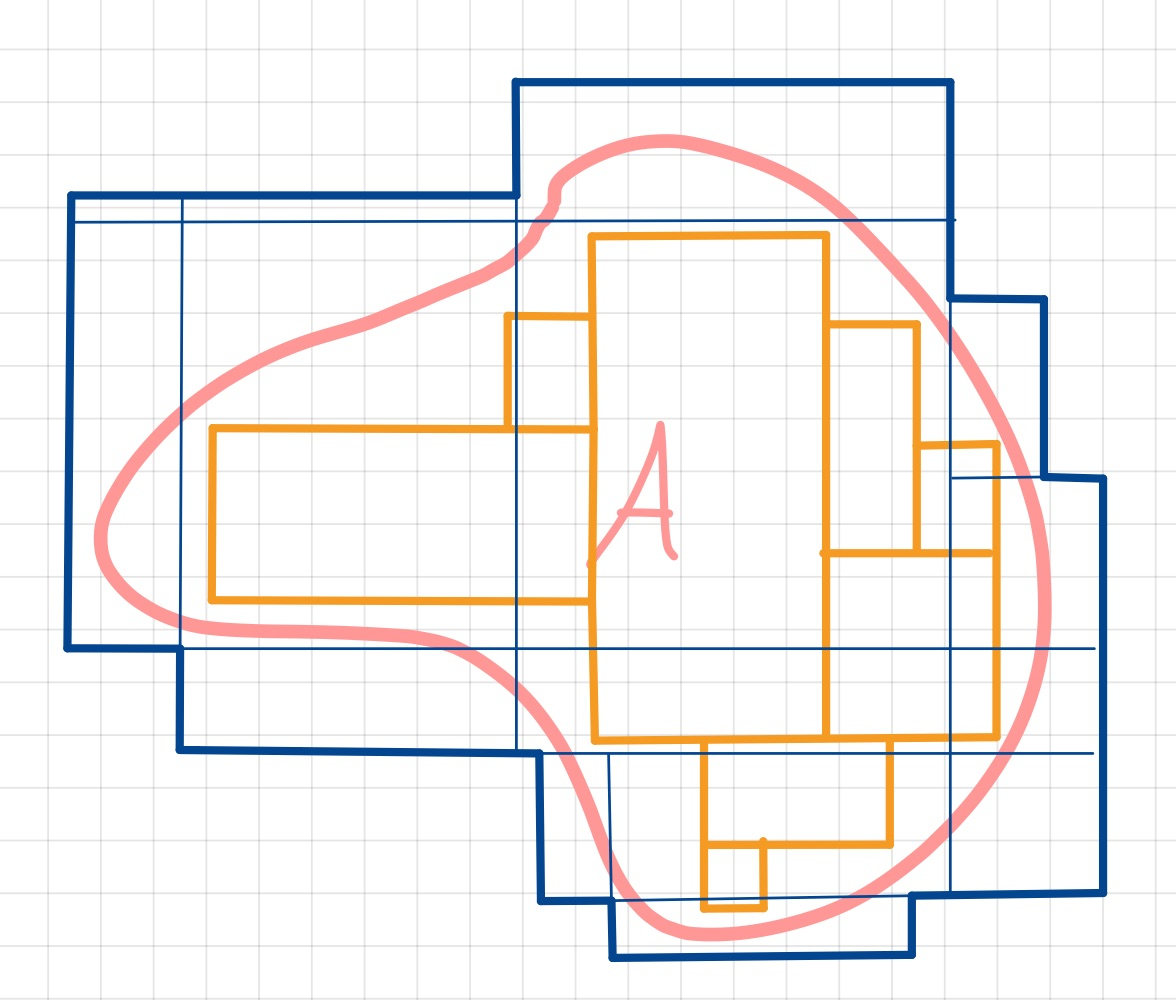
\includegraphics[width=\textwidth]{../\string_build/html/\string_images/jordanmeasure.jpg}
\caption{Visualisierung einer Approximation für das äußere (blau) und das inner (orange) Maß.}\label{\detokenize{masstheorie/masstheorie:id1}}\end{figure}

\par
Die Klasse der Jordan messbaren Mengen ist erneut recht klein. Insbesondere hat dieses Konzept erneut Schwierigkeiten mit abzählbar unendlich großen Mengen umzugehen wie folgendes Beispiel zeigt.
\begin{example}{}{masstheorie/masstheorie:ex:jordan}



\par
Wir betrachten die Menge
\begin{align*}
A = (0,1]\cap \mathbb{Q}
\end{align*}
\par
der rationalen Zahlen im Intervall \([0,1]\). Wir betrachten zunächst das äußere Maß und dazu eine Menge
\begin{align*}
J = \bigcup_{i=1}^N Q_i \supset A,
\end{align*}
\par
mit halboffenen Quader \(Q_1,\ldots,Q_N\). Da aber \(J\) und \((0,1]\) jeweils Elemente aus \(\mathcal{R}_{\text{Q}}\) sind gilt auch
\(L = (0,1]\setminus J \in\mathcal{R}\). Wäre nun \(L\) nicht leer, so gäbe es per Definition der halboffenen Quader eine offene Umgebung
\begin{align*}
U\subset L.
\end{align*}
\par
Da aber \(A\) dicht in \((0,1]\) liegt und somit auch \(J\) führt dies auf einen Widerspruch. Deshalb folgt \(L=\emptyset\) und daher
\begin{align*}
(0,1]\subset J \Rightarrow 1\leq \iota^\ast(A).
\end{align*}
\par
Für das innere Maß betrachten wir
\begin{align*}
J = \bigcup_{i=1}^N Q_i \subset A,
\end{align*}
\par
angenommen \(J\) wäre nicht leer, dann folgt dass eine offenen Umgebung \(U\) existiert s.d.
\begin{align*}
U\subset J.
\end{align*}
\par
Da aber auch die irrationalen Zahlen \(\R\setminus \mathbb{Q}\) dicht in \(\R\) liegen folgt daher
\begin{align*}
\left[U\cap\R\setminus \mathbb{Q} \neq \emptyset\right] 
\Rightarrow 
\left[J \cap \R\setminus \mathbb{Q} \neq \emptyset\right]
\Rightarrow 
\left[J\not\subset \mathbb{Q}\right]
\end{align*}
\par
was im Widerspruch zu \(J\subset A\) steht, daher gilt
\begin{align*}
J=\emptyset\Rightarrow \iota_\ast(J) = 0
\end{align*}
\par
und somit
\begin{align*}
\iota_\ast(J) \neq \iota^\ast(J).
\end{align*}\end{example}

\par
Die Menge der Jordan messbaren Mengen bildet weiterhin keine \(\sigma\) Algebra und daher ist der Jordan Inhalt kein Maß im Sinne von \cref{masstheorie/masstheorie:def:mass}  Dies ist an folgendem Beispiel ersichtlich.
\begin{example}{}{masstheorie/masstheorie:example-20}



\par
Wir wollen den Jordan Inhalt einer Punktmengen \(\{a\}\) für \(a\in\R\) berechnen. Mit der Argumentation aus \cref{masstheorie/masstheorie:ex:jordan} erkennen wir, dass das innere Maß gleich null ist, also
\begin{align*}
\iota_\ast(\{a\}) = 0.
\end{align*}
\par
Für das äußere Maß wählen wir eine Folge von offenen Quadern \(Q_i:= (a-1/i, a] \supset \{a\}\) und erkennen, dass
\begin{align*}
\iota^\ast(\{a\})\leq \lim_{i\to\infty} \lambda^n(Q_i) = \lim_{i\to\infty} 1/i = 0
\end{align*}
\par
und damit ist jede Punktmenge Jordan messbar.

\par
Da aber \(\mathbb{Q}\) abzählbar ist, können wir eine Folge \((q_i)_{i\in\N}\) finden, s.d.
\begin{align*}
A = (0,1]\cap \mathbb{Q} = \bigcup_{i\in\N} \{q_i\},
\end{align*}
\par
die Menge \(A\) lässt sich also als abzählbare Vereinigung von Jordan messbaren Mengen darstellen. Aus \cref{masstheorie/masstheorie:ex:jordan} wissen wir aber, dass \(A\) nicht Jordan messbar ist und somit bildet die Klassen der Jordan messbaren Menge \textbf{keine} \(\sigma\) Algebra.
\end{example}


\subsubsection{Das äußere Lebesgue Maß}
\label{\detokenize{masstheorie/masstheorie:das-auszere-lebesgue-masz}}
\par
Wir der letzte Abschnitt zeigt ist der Begriff der Jordan messbarkeit einerseits zu einschränkend (siehe \cref{masstheorie/masstheorie:ex:jordan}  und andererseits führt er nicht auf eine \(\sigma\) Algebra. Wir werden diesen Begriff nun erweitern indem wir uns zunächst nur auf den äußeren Inhalt konzentrieren.

\begin{emphBox}{}{}{Note:}
\par
Der innere und äußere Inhalt sind intuitiv nicht gleichberechtigt, da das Problem asymmetrisch ist. Konkret ist Subadditivität die inhärente Eigenschaft eines Maßes, da Mengenvereinigungen mehrfach auftretenden Elemente nicht berücksichtigen, während die Addition in \(\R\) für positive Zahlen stets ein größeres Ergebnis liefert. Das äußere Maß ist auf natürliche Weise subadditiv und deshalb zu bevorzugen.
\end{emphBox}
\begin{definition}{}{masstheorie/masstheorie:definition-21}



\par
Das \textbf{äußere Lebesgue Maß} \(\lambda^* \colon 2^{\R^n} \rightarrow [0,\infty]\) ist definiert durch
\begin{align*}
\lambda^*(A) = \inf \left\{ \sum_{k=1}^\infty \mu^n(Q_k) : Q_k \text{ sind halboffene Quader mit } A \subset \bigcup_{k=1}^\infty Q_k \right\}.
\end{align*}\end{definition}

\par
Im Vergleich zum Jordan Inhalt lassen wir nun also unendliche Vereinigungen zu und werten dann Reihen aus überw elche das Infimum gebildet wird. Die erste wichtig Aussage in diesem Kontext geht auf Lebesgue zurück. Der Beweis des Satzes benutzt den Satz von Heine Borel.
\begin{theorem}{(Heine Borel)}{masstheorie/masstheorie:thm:heineborel}



\par
Für eine Menge \(\Omega\subset\R^n\) sind die folgenden beiden Aussagen äquivalent:
\begin{enumerate}

\item {} 
\par
\(\Omega\) ist beschränkt und abgeschlossen.

\item {} 
\par
Jede offene Überdeckung von \(\Omega\) enthält eine endliche Teilüberdeckung.

\end{enumerate}
\end{theorem}

\begin{proof}
 Siehe z.B. \cite{For17}.
\end{proof}

\par
Mit diesem Resultat können wir die folgende Aussage beweisen.
\begin{theorem}{}{masstheorie/masstheorie:thm:lebesgue}



\par
Es sei \(J\in\mathcal{R}_{\text{Q}}\) und \((Q_k)_{k\in\N}\) Folge halboffene Quader mit \(J \subset \bigcup_{k=1}^\infty Q_k\).
Dann gilt
\begin{align*}
\lambda^n(J) = \iota(J) = \leq \sum_{k=1}^\infty \lambda^n(Q_k).
\end{align*}\end{theorem}

\begin{proof}
 Wir zeigen die Aussage zunächst für \(J=Q\) wobei \(Q\) ein halboffener Quader ist.

\par
\textbf{Idee:} Verkleinere \(Q\) und vergrößere die \(Q_i\) um Heine Borel anwenden zu können.

\par
Es sei \(\varepsilon>0\) gegeben. Für \(Q=(a,b]\) können wir einen kleineren halboffenen Quader \(Q_\varepsilon\) wählen, s.d.
\begin{align*}
\overline{Q_\varepsilon} \subset Q\\
\lambda^n(Q_\varepsilon) > \lambda^n(Q) - \varepsilon.
\end{align*}
\par
Beachte, dass der Quader so gewählt wird, dass auch sein Abschluss noch in \(Q\) enthalten ist, die zweite Bedingung gibt eine unter Schranke an wie klein der Quader gewählt werden darf. Man kann leicht nachrechnen, dass ein solcher Quader existiert.

\par
Weiterhin wählen wir für jeden Quader \(Q_k\) einen größeren Quader \(Q_k^\varepsilon\), s.d.,
\begin{align*}
\text{Int}(Q_k^\varepsilon)\supset Q_k\\
\lambda^n(Q_k^\varepsilon) < \lambda^n(Q_k) + \frac{\varepsilon}{2^k},
\end{align*}
\par
wobei \(\text{Int}(\cdot)\) das Innere einer Menge bezeichnet.

\par
Mit dieser Konstruktion gilt
\begin{align*}
\overline{Q_\varepsilon} \subset Q\subset \bigcup_{k\in\N} Q_k \subset 
\bigcup_{k\in\N}\text{Int}(Q_k^\varepsilon)
\end{align*}
\par
daher bilden die Mengen \(\text{Int}(Q_k^\varepsilon)\) eine abzählbare offenen Überdeckung der kompakten Menge \(\overline{Q_\varepsilon}\).
Nach dem Satz von Heine Borel (\cref{masstheorie/masstheorie:thm:heineborel}  existiert somit eine endliche Teilüberdeckung und daher ein \(N\in\N\), s.d.,
\begin{align*}
\overline{Q_\varepsilon}\subset \bigcup_{k=1}^N\text{Int}(Q_k^\varepsilon).
\end{align*}
\par
Für endlich viele Quader können wir nun die Eigenschaften aus \cref{masstheorie/masstheorie:thm:lebesguevolume} benutzen und folgern
\begin{align*}
\lambda^n(Q) -\varepsilon &< \lambda^n(Q_\varepsilon) \leq 
\lambda^n\left(\bigcup_{k=1}^N\text{Int}(Q_k^\varepsilon\right) 
\\&\leq 
\sum_{k=1}^N \lambda^n(Q_k^\varepsilon) < 
\sum_{k=1}^N \lambda^n(Q_k) + \frac{\varepsilon}{2^k} 
\\&\leq
\sum_{k=1}^\infty \lambda^n(Q_k) + \frac{\varepsilon}{2^k} = \sum_{k=1}^\infty \lambda^n(Q_k) +\varepsilon.
\end{align*}
\par
Da \(\varepsilon>0\) beliebig war folgt die Aussage indem wir \(\varepsilon\) gegen \(0\) schicken.

\par
Sei nun \(J\in\mathcal{R}_{\text{Q}}\), wobei \(W_1,\ldots,W_N\) paarweise disjunkte halboffene Quader existieren, s.d.,
\begin{align*}
J = \bigcup_{i=1}^N W_i.
\end{align*}
\par
Dann sehen wir, dass für jedes \(i=1,\ldots,N\) die Folge \((Q_k\cap W_i)_{k\in\N}\) erneut eine Folge halboffener Quader mit
\begin{align*}
W_i \subset \bigcup_{k\in\N} Q_k\cap W_i
\end{align*}
\par
ist und daher können wir den ersten Fall anwenden. Somit folgt
\begin{align*}
\iota(J) = \sum_{i=1}^N \lambda^n(W_i) \leq \sum_{i=1}^N \sum_{k=1}^\infty \lambda^n(W_i\cap Q_k) = 
\sum_{k=1}^\infty\sum_{i=1}^N \lambda^n(W_i\cap Q_k) = \sum_{k=1}^\infty \lambda^n(Q_k).
\end{align*}\end{proof}

\par
Analog zum Lebesgue Inhalt auf \(\mathcal{R}_\text{Q}\) in \cref{masstheorie/masstheorie:thm:lebesguevolume} können wir auch für das äußere Lebesgue Maß ähnliche Eigenschaften zeigen.
\begin{theorem}{(Eigenschaften des äußeren Lebesgue Maßes)}{masstheorie/masstheorie:thm:outerlebesgue}



\par
Das äußere Lebesgue Maß \(\lambda^*\) hat folgende Eigenschaften:

\par
1. \(\lambda^*(\emptyset) = 0\)

\par
2. Für zwei Mengen \(A, B \in \R^n\) mit \(A \subset B\) gilt:
\begin{align*}
\lambda^*(A) \leq \lambda^*(B) \qquad (\text{Monotonie}).
\end{align*}
\par
3. Für eine Folge \((A_k)_{k\in\N}\) von Teilmengen des \(\R^n\) gilt:
\begin{align*}
\lambda^*\left( \bigcup_{k=1}^\infty A_k \right) \leq \sum_{k=1}^\infty \lambda^*(A_k) \qquad (\sigma\!-\!\text{Subadditivität}).
\end{align*}
\par
4. Für \(J\in\mathcal{R}_{\text{Q}}\) gilt,
\begin{align*}
\lambda^*(J) = \iota(J).
\end{align*}
\par
5. Für jede Teilmenge \(A \subset \R^n\) und jeden halboffenen Quader \(Q\) gilt:
\begin{align*}
\lambda^*(A) = \lambda^*(A \setminus Q) + \lambda^*(A \cap Q).
\end{align*}\end{theorem}

\begin{proof}
 \textbf{Ad 1.}

\par
Da \(\emptyset\) ein halboffener Quader ist gilt
\begin{align*}
0\leq \lambda^\ast(\emptyset) \leq \lambda^n(\emptyset) = 0.
\end{align*}
\par
\textbf{Ad 2.}

\par
Es bezeichne
\begin{align*}
\mathcal{C}(B) = \{ (Q_i)_{i\in\N}: Q_i \text{ ist halboffener Quader, für }i\in\N, B\subset \bigcup_{i\in\N} Q_i  \}
\end{align*}
\par
die Menge der möglichen Quaderüberdeckungen. Aus \(A\subset B\) folgt dann \(\mathcal{C}(B) \subset \mathcal{C}(A)\), da jede Überdeckung für \(B\) auch eine Überdeckung für \(A\) ist und daher
\begin{align*}
\lambda^\ast(A) = \inf_{\sum_{i=1}^\infty:(Q_i)_{i\in\N}\in \mathcal{C}(A)} \leq 
\inf_{\sum_{i=1}^\infty:(Q_i)_{i\in\N}\in \mathcal{C}(B)} = \lambda^\ast(B).
\end{align*}
\par
\textbf{Ad 3.}

\par
Sei \(\varepsilon>0\) gegeben. Per Definition des Infimums existiert für jede Menge \(A_k\) eine Folge von halboffenen Quadern \(Q_k^i, i\in\N\), s.d.
\begin{align*}
A_k \subset \bigcup_{i\in\N} Q_i\\
\lambda^\ast(A_k) > \sum_{i=1}^\infty \lambda^n(Q_k^i) - \frac{\varepsilon}{2^k}.
\end{align*}
\par
Dann folgt aber auch, dass
\begin{align*}
\bigcup_{k\in\N} A_k \subset \bigcup_{k\in\N}\bigcup_{i\in\N} Q_k^i
\end{align*}
\par
und da die rechte Seite erneut eine Quaderüberdeckung ist folgt per Definition
\begin{align*}
\lambda^\ast\left(\bigcup_{k\in\N} A_k\right) 
&\leq \sum_{k=1}^\infty\sum_{i=1}^\infty \lambda^n(Q_k^i)\\
&<
\sum_{k=1}^\infty \lambda^\ast(A_k) - \frac{\varepsilon}{2^k} =
\sum_{k=1}^\infty \lambda^\ast(A_k) - \varepsilon.
\end{align*}
\par
Die Aussage folgt indem wir \(\varepsilon\) gegen 0 schicken.

\par
\textbf{Ad 4.}

\par
Es sei \(J\in\mathcal{R}_{\text{Q}}\), per Definition folgt direkt
\begin{align*}
\lambda^\ast(Q)\leq \iota^\ast(Q).
\end{align*}
\par
Mit \cref{masstheorie/masstheorie:thm:lebesgue} folgt aber auch
\begin{align*}
\iota^\ast(Q)\leq \lambda^\ast(Q).
\end{align*}
\par
\textbf{Ad 5.}

\par
Es seien zunächst \(A\) und \(Q\) halboffene Quader, dann ist auch \(A\cap Q\) ein halboffener Quader und wir finden paarweise disjunkte halboffene Quader \(Q_0,\ldots,Q_N\), s.d.
\begin{align*}
A\cap Q = Q_0\\
A = \bigcup_{i=1}^N Q_i
\end{align*}
\par
und damit
\begin{align*}
\lambda^n(A) &= \lambda^n\left(\bigcup_{i=0}^N Q_i\right)\\
&= 
\lambda^n(A\cap Q) + \lambda^n\left(\bigcup_{i=1}^N Q_i\right)\\
&\geq \lambda^n(A\cap Q) + \lambda^n(A\setminus Q) \\
&\geq \lambda^n(A).
\end{align*}
\par
Durch die Abschätzung nah oben und nach unten folgt dann
\begin{align*}
\lambda^n(A) = \lambda^n(A\cap Q) + \lambda^n(A\setminus Q).
\end{align*}
\par
Als nächsten Schritt betrachten wir eine Folge halboffener Quader \((Q_i)_{i\in\N}\mathcal{C}(A)\) und erhalten dann
\begin{align*}
\sum_{i=1}^\infty \lambda^n(Q_i) &= 
\sum_{i=1}^\infty \lambda^n(Q_i\cap Q) + \lambda^n(Q_i\setminus Q)\\
&\overset{2.}{\geq}
\lambda^n(A\cap Q) + \lambda^n(A\setminus Q)
&\overset{2.}{\geq}
\lambda^n(A).
\end{align*}
\par
Nehmen wir das Infimum über \(\mathcal{C}(A)\) folgt
\begin{align*}
\lambda^n(A) \geq \lambda^n(A\cap Q) + \lambda^n(A\setminus Q) \geq 
\lambda^n(A)
\end{align*}
\par
und daher die Behauptung.
\end{proof}

\par
Als Korollar von \cref{masstheorie/masstheorie:thm:lebesgue} und den vorherigen Eigenschaften erhalten wir eine Abschätzung für das äußere Lebesgue Maß sowohl von oben durch den äußeren Jordan Inhalt als auch von unten durch den inneren Jordan Inhalt.
\label{masstheorie/masstheorie:corollary-25}
\begin{emphBox}{}{}{Corollary 5.1}



\par
Es sei \(A\subset\R^n\), dann gilt
\begin{align*}
\iota_\ast(A) \leq \lambda^\ast(A) \leq \iota^\ast(A).
\end{align*}\end{emphBox}

\begin{proof}
 Für jedes Element \(J\in\mathcal{R}_{\text{Q}}\) und beliebige halboffene Quader \(Q_i,\i\in\N\), s.d.,
\begin{align*}
J\subset A\subset \bigcup_{i\in\N} Q_i
\end{align*}
\par
folgt aus \cref{masstheorie/masstheorie:thm:lebesgue} \begin{align*}
\lambda^n(J)\leq \sum_{i=1}^\infty Q_i.
\end{align*}
\par
Dies gilt für jedes \(J\in \mathcal{R}_{\text{Q}}\) mit \(J\subset A\) und daher insbesondere auch für das Supremum, daher
\begin{align*}
\iota_\ast(A) \leq \sum_{i=1}^\infty Q_i.
\end{align*}
\par
Diese Aussage gilt wiederum für eine beliebige Folge halboffener Quader welche \(A\) überdecken und daher auch für das Infimum, also
\begin{align*}
\iota_\ast(A) \leq \lambda^\ast(A).
\end{align*}
\par
Die andere Ungleichung folgt per Definition da jede endliche Überdeckung mit halboffenen Quadern (welche im Infimum für \(\iota^\ast\) betrachtet werden) auch im Infimum über abzählbare Überdeckungen berücksichtigt wird, daher
\begin{align*}
\lambda^\ast(A)\leq\iota^\ast(A).
\end{align*}\end{proof}

\par
Die obige Eigenschaft liefert zusätzlich die Aussage, dass für Jordan messbare Mengen \(A\) gilt
\begin{align*}
\iota(A)\leq\lambda^\ast(A)\leq\iota(A)\Rightarrow \lambda^\ast(A) = \iota(A).
\end{align*}\begin{remark}{(Wirkung von Transformationen auf das äußere Lebesgue Maß)}{masstheorie/masstheorie:rem:transinvariance}



\par
Eine besondere Eigenschaft des äußeren Lebesgue Maßes ist es, dass es \emph{bewegungsinvariant} ist, d.h., dass es unter Translationen und Rotationen den gleichen Wert behält.
Dies ist für viele Anwendungen eine fundamentale Eigenschaft.
Die folgende Bemerkung hält die Wirkung von geometrischen Transformationen auf das äußere Lebesgue Maß fest.

\par
1. Sei \(A \subset \R^n\) eine beliebige Teilmenge und \(a \in \R^n\) ein beliebiger Vektor.
Dann ist das äußere Lebesgue Maß \textbf{translationsinvariant} unter der Wirkung von \(a\), d.h., es gilt
\begin{align*}
\lambda^*(A + a) = \lambda^*(A).
\end{align*}
\par
Außerdem gilt, dass die Teilmenge \(A\) genau dann Lebesgue messbar ist, wenn die verschobene Teilmenge \(A + a\) Lebesgue messbar ist.

\par
2. Sei \(A \subset \R^n\) eine beliebige Teilmenge und \(M \in \R^{n\times n}\) eine beliebige Matrix.
Dann gilt für das äußere Lebesgue Maß der folgende Zusammenhang unter der Wirkung der linearen Transformation \(M\)
\begin{align*}
\lambda^*(MA) = |\!\operatorname{det}(M)| \, \lambda^*(A).
\end{align*}
\par
Das heißt insbesondere, dass das äußere Lebesgue Maß invariant unter Transformationen der orthogonalen Gruppe (z.B. \textbf{Rotationen} und \textbf{Spiegelungen}) ist, da für diese Transformationen \(|\!\operatorname{det}(M)| = 1\) gilt (siehe Kapitel 3.6 in \cite{Ten21}).

\par
Außerdem gilt, dass die Teilmenge \(A\) genau dann Lebesgue messbar ist, wenn die linear transformierte Teilmenge \(MA\) Lebesgue messbar ist.
\end{remark}


\subsubsection{Nullmengen}
\label{\detokenize{masstheorie/masstheorie:nullmengen}}
\par
Eine relevante Klasse von Teilmengen des \(\R^n\) bilden sogenannten \textbf{Lebesgue Nullmengen}.
\begin{definition}{}{masstheorie/masstheorie:definition-27}



\par
Eine Teilmenge \(N \subset \R^n\) eine \textbf{(Lebesgue )Nullmenge}, falls ihr äußeres Lebesgue Maß Null ist, d.h., es gilt
\begin{align*}
\lambda^*(N) = 0.
\end{align*}\end{definition}

\par
Für die Klasse der Nullmengen können wir folgende Eigenschaften zeigen.
\begin{lemma}{(Eigenschaften von Lebesgue Nullmengen)}{masstheorie/masstheorie:lem:eigenschaftenNullmengen}



\par
Für Lebesgue Nullmengen gelten die folgenden Eigenschaften:
\begin{enumerate}

\item {} 
\par
Sei \((N_n)_{n\in\N}\) eine Familie von Nullmengen.
Dann ist auch \(\bigcup_{n\in\N} N_n\) eine Nullmenge.

\item {} 
\par
Alle abzählbare Mengen sind Nullmengen.

\item {} 
\par
Alle Teilmengen von Nullmengen sind Nullmengen.

\end{enumerate}
\end{lemma}

\begin{proof}
 

\par
\textbf{Ad 1.}

\par
Auf Grund der \emph{\(\sigma\) Subadditivität} des äußeren Lebesgue Maßes folgt direkt
\begin{align*}
0 \leq \mu^* \left( \bigcup_{n\in\N} N_n \right) \leq \sum_{n\in\N} \mu^*(N_n) = 0.
\end{align*}
\par
Da \(\mu^* \left( \bigcup_{n\in\N} N_n \right)\) gilt ist also \(\bigcup_{n\in\N} N_n\) auch eine Nullmenge.

\par
\textbf{Ad 2.}

\par
Es sei \(A\subset\R^d\) eine abzählbare Menge, d.h., es existiert eine Folge \((a_k)_{k\in\N}\subset\R^d\), s.d.,
\begin{align*}
A = \bigcup_{k\in\N} a_k.
\end{align*}
\par
Es sei nun \(\varepsilon>0\) gegeben, dann wählen wir die Folge halboffener Quader
\begin{align*}
Q_k := (a_k - \frac{\varepsilon}{2^k},a_k]
\end{align*}
\par
s.d.,
\begin{align*}
A\subset \bigcup_{k\in\N} Q_k.
\end{align*}
\par
Dann folgt aber,
\begin{align*}
\lambda^\ast(A) \leq \sum_{k\in\N} \lambda^n(Q_k) = \sum_{k\in\N} \frac{\varepsilon}{2^k} = \varepsilon.
\end{align*}
\par
Wir können nun \(\varepsilon\) gegen 0 schicken und erhalte die Aussage.

\par
\textbf{Ad 3.}

\par
Es sei \(N\) eine Nullmenge und \(A\subset N\), dann folgt aus der Monotonie
\begin{align*}
0\leq \lambda^\ast(A)\leq \lambda^\ast(N) = 0.
\end{align*}\end{proof}

\par
Intuitiv könnten man meinen, dass lediglich abzählbare MEngen Lebesgue Nullmengen sind, dies ist jedoch nicht der Fall. Ein Beispiel ist die \href{https://de.wikipedia.org/wiki/Cantor-Menge}{canto Menge} welche überabzählbar ist, aber Lebesgue Maß null hat.


\subsubsection{Das äußere Maß ist kein Maß}
\label{\detokenize{masstheorie/masstheorie:das-auszere-masz-ist-kein-masz}}
\par
Für das äußere Lebesgue Maß kann man einige Eigenchaften zeigen (siehe \cref{masstheorie/masstheorie:thm:outerlebesgue}  welche zwar eine Maß erinnern. Der größte Unterschied bisher ist, dass wir nur \(\sigma\) Subadditivität und nicht \(\sigma\) Additivität zeigen konnten. Insbesondere arbeitet das äußere Maß auf der gesamten Potenzmenge \(2^{\R^d}\) und nicht auf einer kleineren \(\sigma\) Algebra, man könnte also vermuten, dass diese Menge zu groß ist um \(\sigma\) Additivität zeigen zu können, was tatsächlich der Fall ist.

\par
Um das zu sehen betrachten wir die sogenannte Vitali Menge auf \(\R\).

\begin{emphBox}{Giuseppe Vitali}{}

\par
\href{https://de.wikipedia.org/wiki/Giuseppe\_Vitali}{Giuseppe Vitali} (geboren 26. August 1875 in Ravenna; gestorben 29. Februar 1932 in Bologna) war ein italienischer Mathematiker.
\end{emphBox}

\par
Für zwei Punkte \(x,y\in\R\) definiert man die Äquivalenzrelation
\begin{align*}
x \sim y \quad \Leftrightarrow \quad x-y \in \Q.
\end{align*}
\par
d.h. zwei Punkte gehören der selben Äquivalenzklasse an sofern ihre Differenz rational ist. Es gilt also
\begin{align*}
[x] = \{y: y-x\in\Q\}
\end{align*}
\par
jede Klasse \([x]\) ist abzählbar und \([0] = \Q\). Falls \([x]\cap [y]\neq \emptyset\), so folgt, dass ein \(z\in[x]\cap [y]\) existiert und damit
\begin{align*}
\left.
\begin{matrix}
z-x\in\Q\\
z-y\in\Q\\
\end{matrix}
\right\}
\Rightarrow x-y\in\Q\Rightarrow [x]=[y],
\end{align*}
\par
daher sind zwei Äquivalenzklassen entweder gleich oder disjunkt. Da aber
\begin{align*}
\R = \bigcup_{x\in\R} [x]
\end{align*}
\par
gilt, muss es überabzählbar viele disjunkte Äquivalenzklassen geben, ansonsten wäre \(\R\) selbst abzählbar. Mithilfe des \href{https://de.wikipedia.org/wiki/Auswahlaxiom}{Auswahl Axioms} können wir nun für jede einzelne Äquivalenzklasse einen Repräsentanten wählen, wobei wir die Menge der Repräsentanten \(V\) als \textbf{Vitali Menge} bezeichnen. Zwei Elemente \(x,y\in V, x\neq y\) unterscheiden sich stets um eine irrationale Zahl, denn
\begin{align*}
x-y\in\Q \Rightarrow [x] = [y]
\end{align*}
\par
ist ein Widerspruch zur Konstruktion.

\par
Es sei nun \((q_k)_{k\in\N}\) eine Abzählung der rationalen Zahlen und definiere die verschobenen Vitali Mengen
\begin{align*}
V_k :=\{x+q_k: x\in V\}.
\end{align*}\begin{lemma}{}{masstheorie/masstheorie:lemma-29}



\par
Mit den obigen Definitionen gilt
\begin{enumerate}

\item {} 
\par
\(\lambda^\ast(V) = \lambda^\ast(V_k)\) für alle \(k\in\N\),

\item {} 
\par
\(V_k\cap V_l=\emptyset\) für \(k\neq l\),

\item {} 
\par
\(\bigcup_{k\in\N} V_k = \R\).

\end{enumerate}
\end{lemma}

\begin{proof}
 

\par
\textbf{Ad 1.}

\par
Diese Tatsache folgt, da das äußere Lebesgue Maß Translationsinvariant ist, siehe \cref{masstheorie/masstheorie:rem:transinvariance} 

\par
\textbf{Ad 2.}

\par
Für \(x,y\in V\) gilt
\begin{align*}
x + q_k = y + q_l&\Rightarrow x-y\in\Q\\
\Rightarrow [x]=[y]&\Rightarrow x=y\\
\Rightarrow q_k=q_l&\Rightarrow k=l
\end{align*}
\par
wobei wir in der zweiten Zeile erneut ausnutzen, dass die Elemente aus \(V\) jeweils disjunkte Äquivalenzklassen erzeugen.

\par
\textbf{Ad 3.}

\par
Trivialerweise gilt
\begin{align*}
\bigcup_{k\in\N} V_k \subset \R.
\end{align*}
\par
Andererseits sei \(x\in\R\) dann existiert \(v\in V\) s.d. \([v] = [x]\). Somit gilt \(x-v\in\Q\) und es existiert \(k\in\N\), s.d.
\begin{align*}
q_k = x-v.
\end{align*}
\par
Somit folgt \(x=v+q_k\in V_k\) und daher \(x\in\bigcup_{k\in\N} V_k\).
\end{proof}

\par
Mithilfe einer Vitali Menge können wir nun die \(\sigma\) Additivität des äußeren Lebesgue Maßes zum Widerspruch führen.
\begin{lemma}{}{masstheorie/masstheorie:lemma-30}



\par
Das äußere Lebesgue Maß \(\lambda^\ast\) ist nicht \(\sigma\) Additiv auf \(2^{\R}\).
\end{lemma}

\begin{proof}
 \textbf{Annahme}: Das äußere Lebesgue Maß sei \(\sigma\) Additiv auf \(2^{\R}\).

\par
Die Mengen \(V_k\) sind paarweise disjunkt und überdecken \(\R\), daher folgt
\begin{align*}
0<\lambda^\ast(\R) = \lambda^\ast(\bigcup_{k\in\N} V_k) = \sum_{k\in\N} \lambda^\ast(V_k) = \sum_{k\in\N} \lambda^\ast(V)
\end{align*}
\par
und daher \(\lambda^\ast(V)>0\). Diese Folgerung wollen wir nun zum Widerspruch führen. Dazu betrachten wir die folge halboffener Quader \(Q_k:=(k,k]\) und erkennen unter Ausnutzung \textbf{endlicher} Additivität, dass
\begin{align*}
\lambda^\ast(V) \geq \lambda^\ast\left(V \cap \bigcup_{k=1}^N Q_k\right) = 
\sum_{k=1}^N \lambda^\ast(V\cap Q_k).
\end{align*}
\par
Somit folgt mithilfe der \(\sigma\) Subadditivität
\begin{align*}
\lambda^\ast(V) \geq \sum_{k=1}^\infty \lambda^\ast(V\cap Q_k) \geq
\lambda^\ast\left(\bigcup_{k\in\N} V\cap Q_k\right) = \lambda^\ast(V).
\end{align*}
\par
Da wir \(\lambda^\ast(V)>0\) folgern konnten, muss daher ein \(N\in\N\) existieren, s.d.,
\begin{align*}
\lambda^\ast(V\cap Q_N) >0.
\end{align*}
\par
Analog zum Beweis, dass die \(V_k\) paarweise disjunkt sind, folgert man auch, dass die Mengen \(\frac{1}{m}+(V\cap Q_N)\) für verschieden \(m\in\N\) paarweise disjunkt sind und wegen der Translationsinvarianz folgt
\begin{align*}
\lambda^\ast(\frac{1}{m}+(V\cap Q_N)) = \lambda^\ast((V\cap Q_N)) >0.
\end{align*}
\par
Wir erkennen allerdings, dass
\begin{align*}
\bigcup_{m\in\N} \frac{1}{m}+(V\cap Q_N) \subset (-N,N+1]
\end{align*}
\par
und nutzen wir nun erneut die angenommene \(\sigma\) Additivität so erhalten wir
\begin{align*}
\infty = \sum_{m=1}^\infty \lambda^\ast(\frac{1}{m}+(V\cap Q_N)) = 
\lambda^\ast\left(\bigcup_{m\in\N}  \frac{1}{m}+(V\cap Q_N) \right)\leq 
\lambda^\ast((-N,N+1]) = 2N + 1
\end{align*}
\par
und somit
\begin{align*}
\infty \leq 2N + 1
\end{align*}
\par
was ein Widerspruch ist. Daher ist die Annahme der \(\sigma\) Additivität falsch.
\end{proof}

\par
Ähnliche Konstruktionen können auch allgemein für \(\R^n\) durchgeführt werden. Man hat allgemein die Aussage, dass \(\lambda^\ast\) auf \(\R^n\) \textbf{kein} Maß ist.


\subsubsection{Das Lebesgue Maße}
\label{\detokenize{masstheorie/masstheorie:das-lebesgue-masze}}
\par
Der vorherige Abschnitt zeigt, dass die Potenzmenge \(2^{\R^n}\) zu groß ist, d.h. auf dieser \(\sigma\) Algebra ist \(\lambda^\ast\) kein Maß. Deshalb wollen wir nun eine Klasse messbarer Mengen definieren, welche dann eine kleinere \(\sigma\) Algebra liefert.
\begin{remark}{(Das Jordan Konzept)}{masstheorie/masstheorie:remark-31}



\par
Eine mögliche Idee um messbare Mengen zu definieren haben wir bereits beim Jordan Inhalt kennengelernt. Hierbei wird zusätzlich zum äußeren Mein inneres definiert. Beim Übergang vom äußeren Jordan Inhalt zum äußeren Lebesgue Maß werden endliche Vereinigungen durch unendliche ersetzt, weshalb man versuchen könnte, das nun auch hier zu tun, indem man das innere Lebesgue Maß auch über unendliche Vereinigungen definiert
\begin{align*}
\lambda_\ast(A) := \sup\left\{\sum_{i=1}^\infty Q_i: \bigcup_{i\in\N} Q_i \subset A, Q_i\text{ disjunkte halboffener Quader}\right\}.
\end{align*}
\par
Offensichtlich folgt mit dieser Definition
\begin{align*}
\iota_\ast(A)\leq \lambda_\ast(A)
\end{align*}
\par
da das Supremum über mehr Ausschöpfungen gebildet wird. Nun sei aber \(Q_i\) eine beliebiger Folge halboffener Quader, welche \(A\) von innen ausschöpfen, dann gilt für jedes \(N\in\N\)
\begin{align*}
\iota_\ast(A) \geq \sum_{i=1}^N \lambda^n(Q_i)
\end{align*}
\par
und daher
\begin{align*}
\iota_\ast(A)\geq \sum_{i=1}^\infty \lambda^n(Q_i).
\end{align*}
\par
Diese Ungleichung erhalten wir deshalb so einfach, da für jedes \(N\in\N\) auch \(\bigcup_{i=1}^N Q_i\subset A\) gilt. Beim äußern Maßen konnten wir aber andersherum nicht einfach aus \(A\subset \bigcup_{i=1}^\infty W_i\) auch \(A\subset \bigcup_{i=1}^N W_i\) folgern.

\par
Da die obige Ungleichung für beliebig Folgen halboffener Quader gilt, folgt
\begin{align*}
\iota_\ast(A) \geq \lambda_\ast(A).
\end{align*}
\par
Wir erkennen also, dass für das innere Maß keinen Unterschied macht ob wir endliche oder unendliche Vereinigungen betrachten.

\par
Würden wir Messbarkeit über die Bedingung
\begin{align*}
\lambda_\ast(A)=\lambda^\ast(A)
\end{align*}
\par
definieren erhielten wir erneut keine \(\sigma\) Algebra. Denn für die Menge \(A=[0,1]\setminus\Q\) gilt
\begin{align*}
J\in\mathcal{R}_{\text{Q}}, J\subset A\Rightarrow J=\emptyset
\end{align*}
\par
und daher \(\lambda_\ast(J) = 0\). Der Trick die Menge mit kleinen Quadern zu approximieren wie beim äußeren Maß funktioniert auch nicht, da wir in diesem Fall jeweils die Teilmengen Bedingung verletzt wäre.

\par
Es gilt aber
\begin{align*}
\lambda^\ast(A) = \lambda^\ast([0,1]) - \underbrace{\lambda^\ast(\Q)}_{=0} = 1
\end{align*}
\par
und daher wäre \(A\) nicht messbar, obwohl sowohl \(\Q\), als auch \([0,1]\) messbar wären. Damit hätten wir erneut keine \(\sigma\) Algebra konstruiert.
\end{remark}

\par
Es gibt verschiedene Ansätze Lebesgue Messbarkeit zu definieren (welche alle äquivalent sind), wir wählen im Folgenden das Konzept von
Carathéodory.

\begin{emphBox}{Constantin Carathéodory}{}

\par
\href{https://de.wikipedia.org/wiki/Constantin\_Carath\%C3\%A9odory}{Constantin Carathéodory} (Geboren 13. September 1873 in Berlin; Gestorben 2. Februar 1950 in München) war ein Mathematiker griechischer Herkunft.
\end{emphBox}
\begin{definition}{}{masstheorie/masstheorie:definition-32}



\par
Wir nennen eine Teilmenge \(A \subset \R^n\) \textbf{Lebesgue messbar}, genau dann wenn für alle Teilmengen \(E \subset \R^n\) gilt:
\begin{align*}
\lambda^*(E) = \lambda^*(E \cap A) + \lambda^*(E \setminus A).
\end{align*}
\par
Wir notieren die Menge der Lebesgue messbaren Mengen als
\begin{align*}
\mathcal{A} = \lbrace A \subset \R^n : A \text{ ist Lebesgue-messbar } \rbrace
\end{align*}
\par
Wir definieren das \textbf{Lebesgue Maß} \(\lambda \colon \mathcal{A} \rightarrow [0,\infty]\) messbarer Mengen durch
\begin{align*}
\lambda(A) = \lambda^*(A).
\end{align*}\end{definition}
\begin{remark}{}{masstheorie/masstheorie:remark-33}



\par
Es ist wichtig zu bemerken, dass diese Bedingung eine Einschränkung ist, da das äußere Lebesgue Maß \textbf{nicht} additiv ist auf \(2^{\R^n}\), es gilt lediglich
\begin{align*}
\lambda^*(E) \leq \lambda^*(E \cap A) + \lambda^*(E \setminus A).
\end{align*}
\par
für alle \(A,E\subset\R^d\). Aus diesem Grund scheint die Einschränkung sinnvoll zu sein um Additivität zu erhalten.
\end{remark}

\par
Wir betrachten im Folgenden verschiedene Beispiele messbarer Mengen, was zeigt, dass \(\mathcal{A}\neq \emptyset\).
\begin{lemma}{(Lebesgue messbare Mengen)}{masstheorie/masstheorie:thm:lebesguemes}


\begin{enumerate}

\item {} 
\par
Jede Lebesgue Nullmenge ist Lebesgue messbar, insbesondere ist \(\emptyset\) Lebesgue messbar.

\item {} 
\par
Jeder halboffene Quader ist messbar.

\end{enumerate}
\end{lemma}

\begin{proof}
 ** Ad 1.**

\par
Es sei \(N\) eine Lebesgue Nullmenge und \(E\subset\R^d\), dann gilt
\begin{align*}
\lambda^\ast(E) \leq \underbrace{\lambda^\ast(E\cap\N)}_{=0} + \lambda^\ast(E\setminus N)\leq
 \lambda^\ast(E)
\end{align*}
\par
und daher \(\lambda^\ast(E) = \lambda^\ast(E\cap\N) + \lambda^\ast(E\setminus N)\).

\par
\textbf{Ad 2.}

\par
Folgt aus \cref{masstheorie/masstheorie:thm:outerlebesgue} Eigenschaft 4.
\end{proof}

\par
Weiterhin erhält man über den Begriff der Lebesgue messbarkeit endlich die erhoffte \(\sigma\) Algebra Struktur.
\begin{lemma}{}{masstheorie/masstheorie:lemma-35}



\par
Die Klasse der Lebesgue messbaren Mengen \(\mathcal{A}\) bildet eine \(\sigma\) Algebra.
\end{lemma}

\begin{proof}
 1. Von \cref{masstheorie/masstheorie:thm:lebesguemes} erhalten wir zunächst, dass \(\emptyset\in\mathcal{A}\).

\par
2. Weiterhin sei \(A\in\mathcal{A}\) messbar und \(E\subset\R^d\) beliebig, dann gilt
\begin{align*}
\lambda^\ast(E) = \lambda^\ast(\underbrace{A\cap E}_{=E\setminus A^C}) + \lambda^\ast(\underbrace{E\setminus A}_{=E\cap A^C}) = 
\lambda^\ast(E\setminus A^C) + \lambda^\ast(E\cap A^c)\end{align*}
\par
und daher ist auch \(A^C\in\mathcal{A}\).

\par
3. Wir zeigen zunächst, dass \(\mathcal{A}\) unter endlichen Vereinigungen, Schnitten und Differenzen abgeschlossen ist.

\par
Es seien \(A,B\in\mathcal{A}\) und \(E\subset\R^d\) dann gilt
\begin{align*}
\lambda^\ast(E) &= \lambda^\ast(E\cap A) + \underbrace{\lambda^\ast(E\setminus A)}_{\text{wende Messbarkeit von} B\text{ an}}\\
&=\lambda^\ast(E\cap A) + \lambda^\ast((E\setminus A)\cap B) + \lambda^\ast((E\setminus A)\setminus B)\\
&=
\underbrace{\lambda^\ast(E\cap (A\cup B)\cap A) + \lambda^\ast((E\cap A\cup B)\setminus A)}_{\text{wende Messbarket von } A \text{ an}} + \lambda^\ast(E\setminus(A\cup B))\\
&=
\lambda^\ast(E\cap (A\cup B)) + \lambda^\ast(E\setminus(A\cup B))
\end{align*}
\par
und daher ist \(A\cup B\) messbar. Weiterhin folgt \(A\cap B = (A^C\cup B^C)^C\in\mathcal{A}\) und daher auch \(A\cap B\in\mathcal{A}\). Außerdem gilt \(A\setminus B = A\cap B^C\) und somit auch \(A\setminus B\in\mathcal{A}\).

\par
4. Sei nun \(A_i\in\mathcal{A}\) für \(i\in\N\) eine \textbf{disjunkte} Folge von Mengen und setze \(A=\bigcup_{i\in\N} A_i\). Unter Ausnutzung von \(A_1\in\mathcal{A}\) haben wir für \(E\subset\R^d\)
\begin{align*}
\lambda^\ast(E\cap (A_1\cup A_2)) &= \lambda^\ast(E\cap(A_1\cup A_2)\cap A_1) + \lambda^\ast(E\cap(A_1\cup A_2)\setminus A_1)\\
&=
\lambda^\ast(E\cap A_1) + \lambda^\ast(E\cap A_2)
\end{align*}
\par
und somit gilt für endliche Vereinigungen
\begin{align*}
\lambda^\ast(E\cap \bigcup_{i=1}^N A_i) = \sum_{i=1}^N \lambda^\ast(E\cap A_i).
\end{align*}
\par
Mit Monotonie folgt dann für jedes \(N\in\N\)
\begin{align*}
\lambda^\ast(E\cap A)\geq \lambda^\ast(E\cap \bigcup_{i=1}^N A_i) = \sum_{i=1}^N \lambda^\ast(E\cap A_i)
\end{align*}
\par
und daher mit der \(\sigma\) Subadditivität
\begin{align}\label{equation:masstheorie/masstheorie:eq:LebesgueAlgebra}
\lambda^\ast(E\cap A) \geq \sum_{i=1}^\infty \lambda^\ast(E\cap A_i)\geq \lambda^\ast\left(\bigcup_{i\in\N} E\cap A_i\right) = \lambda^\ast(E\cap A).
\end{align}
\par
Weiterhin wissen wir nach 3., dass endliche Vereinigungen messbarer Mengen messbar sind, daher
\begin{align*}
\lambda^\ast(E) &= \lambda^\ast\left(E\cap \bigcup_{i=1}^N A_i\right) + \lambda^\ast\left(E\setminus \bigcup_{i=1}^N A_i\right)\\
&\geq
\sum_{i=1}^N \lambda^\ast(E\cap A_i) + \lambda^\ast(E\setminus A)
\end{align*}
\par
für alle \(N\in\N\) und somit
\begin{align*}
\lambda^\ast(E)\geq \sum_{i=1}^\infty \lambda^\ast(E\cap A_i) + \lambda^\ast(E\setminus A)\geq 
\lambda^\ast(E\cap A) + \lambda^\ast(E\setminus A) \geq \lambda^\ast(E).
\end{align*}
\par
Daraus schließen wir mit , dass {\color{red}\bfseries{}:eqref:`eq:LebesgueAlgebra`}
\begin{align*}
\lambda^\ast(E) = \sum_{i=1}^\infty \lambda^\ast(E\cap A_i) + \lambda^\ast(E\setminus A) =
\lambda^\ast(E\cap A) + \lambda^\ast(E\setminus A).
\end{align*}
\par
5.\textbackslash{} Es bleibt die Aussage für eine belibige nicht notwendigerweise disjunkte Folge \(A_i\in\mathcal{A}, i\in\N\) zu zeigen. Dazu definieren wir die Mengen \(B_1:=A_1\),
\begin{align*}
B_k := A_i\setminus \left(\bigcup_{i=1}^k B_i  \right)
\end{align*}
\par
wobei wir erkennen, dass die \(B_i\) paarweise disjunkt sind und insbesondere gilt
\begin{align*}
\bigcup_{k\in\N} B_k = \bigcup_{i\in\N} A_i.
\end{align*}
\par
Nach 4. ist damit auch diese Vereinigung messbar.
\end{proof}

\par
Mit dieser Aussage können wir weitere messbare Mengen identifizieren.
\begin{lemma}{}{masstheorie/masstheorie:thm:lebesgueOffenAbgeschlossen}



\par
Offene und abgeschlossene Teilmengen des \(\R^n\) sind Lebesgue messbar.
\end{lemma}

\begin{proof}
 Es sei \(U\subset\R^d\) offen, wir betrachten die Menge
\begin{align*}
\bigcup_{a,b\in \Q^d, (a,b]\subset U} (a,b]\subset U
\end{align*}
\par
Sei nun \(x\in U\), dann existiert auch \(a,b\in\Q^d\), s.d. \(x\in(a,b]\subset U\) und somit \(x\in\bigcup_{a,b\in \Q^d, (a,b]\subset U}\), woraus wir schließen
\begin{align*}
\bigcup_{a,b\in \Q^d, (a,b]\subset U} (a,b] = U.
\end{align*}
\par
Somit ist \(U\) abzählbare Vereinigung messbarer Mengen und daher selbst messbar.

\par
Abgeschlossene Mengen sind als Komplemente offener und daher messbarer Mengen, selbst messbar.
\end{proof}

\par
Da wir nun eine \(\sigma\) Algebra zu Verfügung haben können wir ein Maß definieren.

\begin{emphBox}{}{}
\par
ToDo
\end{emphBox}
\begin{theorem}{(Regularität des Lebesgue Maßes)}{masstheorie/masstheorie:theorem-37}



\par
Das Lebesgue Maß ist von außen und innen regulär im Sinne von \cref{masstheorie/masstheorie:def:regularitaet}  d.h., für jede Lebesgue messbare Teilmenge \(A \subset \R^n\) gilt

\par
1. für jedes \(\epsilon > 0\) existiert eine offene Menge \(U\) mit \(A \subset U\) für die gilt \(\mu(U \setminus A) < \epsilon\),

\par
2. für jedes \(\epsilon > 0\) existiert eine abgeschlossene Menge \(F\) mit \(F \subset A\) für die gilt \(\mu(A \setminus F) < \epsilon\).
\end{theorem}

\begin{proof}
 ToDo.
\end{proof}
\begin{theorem}{(Charakterisierung Lebesgue messbarer Mengen)}{masstheorie/masstheorie:theorem-38}



\par
Die folgenden drei Aussagen sind äquivalent, so dass sie eine Charakterisierung der Lebesgue messbaren Mengen darstellen.

\par
1. Eine Teilmenge \(A \subset \R^n\) ist Lebesgue messbar.

\par
2. Für jedes \(\epsilon > 0\) existiert eine offene Menge \(U\) und eine abgeschlossene Menge \(F\), so dass \(F \subset A \subset U\) und es gilt \(\mu(U \setminus F) < \epsilon\).

\par
3. Für jedes \(\epsilon > 0\) existiert eine offene Menge \(U\) mit \(A \subset U\) für die gilt \(\mu(U \setminus A) < \epsilon\).
\end{theorem}

\begin{proof}
 ToDo
\end{proof}

\par
Man kann für die Borel \(\sigma\) Algebra von \(\R^n\) zeigen, dass gilt
\begin{align*}
\B(\R^n) = \sigma(\lbrace A \subset \R^n \text{ offen }\rbrace) ) = \sigma(\lbrace A \subset \R^n \text{ abgeschlossen }\rbrace)
\end{align*}
\par
Die letzte Gleichung gilt, da \(\sigma\) Algebren abgeschlossen unter Komplementbildung sind.
Zusammen mit \cref{masstheorie/masstheorie:thm:lebesgueOffenAbgeschlossen} folgt dann schon, dass die Borel \(\sigma\) Algebra \(\B(\R^n)\) eine Teilmenge der Lebesgue messbaren Mengen ist.
Der folgende Satz zeigt, dass es eine echte Teilmenge ist indem er den Unterschied der Mengen als Lebesgue Nullmengen charaterisiert.
\begin{theorem}{}{masstheorie/masstheorie:theorem-39}



\par
Eine Teilmenge \(A \subset \R^n\) ist genau dann Lebesgue messbar, wenn eine Teilmenge \(B \in \B(\R^n)\) und eine Nullmenge \(N \subset \R^n\) existiert, so dass \(A = B \cup N\) ist, wobei \(B\cap N=\emptyset\).
\end{theorem}

\begin{proof}
 ToDo
\end{proof}


\section{Lebesgue Integral}
\label{\detokenize{masstheorie/lebesgue_integral:lebesgue-integral}}\label{\detokenize{masstheorie/lebesgue_integral::doc}}
\par
Anhand des in ?? konstruirten MAßes wollen wir nun einen neuen Begriff des Integrals herleiten. Unsere Motivation hierbei war anstatt den Definitionsbereich, den Bildbereich einer Funktion \(f:\Omega\to\R\) zu zerteilen. Dies führt auf das Problem, dass man Urbildern
\begin{align*}
f^{-1}(I)
\end{align*}
\par
für Mengen \(I\subset\R\) ein Maß zuordnen muss. Dies soll im Folgenden mithilfe des Lebesgue Maßes geschehen. Um \(f^{-1}(I)\) allerdings im Lebesgue Maß auswerten zu können, müssen wir voraussetzen, dass diese Menge messbar ist. Dies führt auf spezielle Anforderungen an die Funktion \(f\).


\subsection{Messbare Funktionen}
\label{\detokenize{masstheorie/lebesgue_integral:messbare-funktionen}}
\par
Wir beginnen mit der Definition von messbaren Funktionen. Wir benutzen hierbei den Begriff eines \textbf{Messraums} der anders als ein MAßraum nur eine Grundmenge und eine \(\sigma\) Algebra voraussetzt und kein Maß beinhaltet.
\begin{definition}{}{masstheorie/lebesgue_integral:definition-0}



\par
Es seien \((\Omega_1,\Sigma_1), (\Omega_1,\Sigma_1)\) zwei Messräume und \(f:\Omega_1\to\Omega_2\) eine Funktion, dann nennen wir \(f\) \textbf{messbar}, falls
\begin{align*}
f^{-1}(A)\in\Sigma_1\quad\forall A\in\Sigma_2
\end{align*}\end{definition}

\par
Für ein Teilmengensystem \(\mathcal{C}\subset 2^{\Omega_2}\) benutzten wir auch die Schreibweise
\begin{align*}
f^{-1}(\mathcal{C}) = \{ f^{-1}(C): C\in\mathcal{C}\},
\end{align*}
\par
womit sich die Messbarkeit einer Funktion äquivalent auch durch die Bedingung
\begin{align*}
f^{-1}(\Sigma_2)\subset\Sigma_1
\end{align*}
\par
schreiben lässt. In diesem Kapitel wollen wir speziell Funktionen \(f:\Omega\to\overline{\R}\) betrachten wobei \(\Omega\subset\R^d\). Hierbei nennen wir \(f\) \textbf{Borel messbar}, falls
\begin{align*}
f^{-1}(\mathcal{B}(\overline{\R}))\subset \mathcal{B}(\R^d).
\end{align*}
\par
Analog nennen wir \(f\) \textbf{Lebesgue messbar}, falls
\begin{align*}
f^{-1}(\mathcal{B}(\overline{\R}))\subset \mathcal{A}.
\end{align*}
\par
Eine wichtige Aussage in dem Kontext von messbaren Funktionen ist die Tatsache, dass sich Urbild mit dem \(\sigma\) Operator vertauschen lässt, wobei für \(\mathcal{C}\subset 2^\Omega\) die Menge \(\sigma(\mathcal{C})\) gerade die kleinste \(\sigma\) Algebra ist welche \(\mathcal{C}\) enthält siehe ??.
\begin{lemma}{}{masstheorie/lebesgue_integral:lemma-1}



\par
Es sei \(f:\Omega_1\to\Omega_2\) eine Funktion und \(\mathcal{C}\subset 2^{\Omega_2}\) ein Teilmengensystem, dann gilt
\begin{align*}
f^{-1}(\sigma(\mathcal{C})) = \sigma(f^{-1}(\mathcal{C})).
\end{align*}\end{lemma}

\begin{proof}
 ToDo
\href{https://www.fau.tv/clip/id/40563}{Vorlesung} ab 29:52.
\end{proof}

\par
Mit diesem Lemma können wir folgende Beziehungen zeigen.
\begin{lemma}{}{masstheorie/lebesgue_integral:lemma-2}


\begin{enumerate}

\item {} 
\par
Borel messbare Funktionen sind Lebesgue messbar

\item {} 
\par
Stetige Funktionen sind Borel messbar.

\end{enumerate}
\end{lemma}

\begin{proof}
 ToDo
\href{https://www.fau.tv/clip/id/40563}{Vorlesung} ab 17:12
\end{proof}


\subsection{Charakterisierung über Niveaumengen}
\begin{remark}{}{\detokenize{masstheorie/lebesgue_integral:charakterisierung-uber-niveaumengen}}\label{masstheorie/lebesgue_integral:remark-3}



\par
1. Konkatenation von messbaren Funktionen ist wieder eine messbare Funktion.

\par
2. Summen, Produkte, Quotienten, Maxima und Minima endlich vieler reellwertiger messbarer Funktionen sind wieder messbar.

\par
3. Sei \((f_n)_{n \in \N}\) mit \(f_n \colon \Omega \subset \R^n \rightarrow \R\) eine Folge von messbaren Funktionen.
Dann sind \(\inf(f_n), \sup(f_n), \lim\inf (f_n)\) und \(\lim\sup (f_n)\) auch messbar.
\end{remark}


\subsection{Das Lebesgue Integral}
\label{\detokenize{masstheorie/lebesgue_integral:das-lebesgue-integral}}
\par
ToDo Definition
\begin{theorem}{}{masstheorie/lebesgue_integral:theorem-4}



\par
Sei \(f \colon \Omega \subset \R^n \rightarrow [0,\infty]\) eine Lebesgue messbare Funktion.
Dann existiert eine monoton wachsende Folge \((T_n)_{n_\in N}\) von Treppenfunktionen mit
\begin{align*}
T_n|_{D^c} = 0 \qquad \text{ und } \qquad T_n \nearrow f,
\end{align*}
\par
d.h., es gilt
\begin{align*}
\lim_{n\rightarrow \infty} T_n(x) = f(x) \qquad \text{ und } \qquad T_{n+1}(x) \geq T_n(x).
\end{align*}\end{theorem}

\begin{proof}
 ToDo
\end{proof}
\begin{definition}{}{masstheorie/lebesgue_integral:definition-5}



\par
1. Für Lebesgue messbare Mengen \(A_i, i=1,\ldots,N\) und nicht negative Koeffizienten \(\alpha_i, i=1,\ldots,N\) definieren wir das \textbf{Lebesgue Integral} einer positiven \emph{Treppenfunktion} \(T = \sum_{i=1}^N \alpha_i \chi_{A_i}\) als
\begin{align*}
\int \mu(\mathrm{d}x) f(x) = \sum_{i=1}^N \alpha_i \mu(A_i).
\end{align*}
\par
2. Sei \((T_n)_{n\in\N}\) eine monoton wachsende Folge von Treppenfunktionen mit
\begin{align*}
T_n|_{D^c} = 0 \qquad \text{ und } \qquad T_n \nearrow f
\end{align*}
\par
und \(f \colon D \rightarrow \overline{R}\) eine positive, \emph{Lebesgue messbare Funktion}.
Dann ist das \textbf{Lebesgue Integral} von \(f\) definiert als
\begin{align*}
\int_D \mu(\mathrm{d}x) f(x) = \lim_{n\rightarrow \infty} \int \mu(\mathrm{d}x) f_n(x) = \sup_n \int \mu(\mathrm{d}x) f_n(x) \in [0,\infty].
\end{align*}\end{definition}
\begin{theorem}{(Eigenschaften des Lebesgue Integrals)}{masstheorie/lebesgue_integral:theorem-6}



\par
Das Lebesgue Integral ist \emph{wohldefiniert}, d.h., sein Wert ist unabhängig von der gewählten Folge von Treppenfunktionen \((T_n)_{n\in\N}\).
Darüber hinaus ist das Lebesgue Integral \emph{linear} und \emph{monoton}, d.h., für nichtnegative, Lebesgue messbare Funktionen \(f,g \geq 0\) gilt
\begin{align*}
\int \mu(\mathrm{d}x)(f(x) + \lambda g(x)) = \left( \int \mu(\mathrm{d}x) f(x) \right) + \lambda \left( \int \mu(\mathrm{d}x) g(x) \right)\\
f \leq g \quad \Rightarrow \quad \int \mu(\mathrm{d}x) f(x) \leq \int \mu(\mathrm{d}x) g(x).
\end{align*}\end{theorem}

\begin{proof}
 ToDo
\end{proof}
\begin{definition}{}{masstheorie/lebesgue_integral:definition-7}



\par
Sei \(f \colon \R^n \rightarrow \R\) eine Lebesgue messbare Funktion.
Wir nennen die Funktion \(f\) \textbf{Lebesgue integrierbar}, genau dann wenn gilt
\begin{align*}
\mu(|f|) < +\infty
\end{align*}
\par
Falls die Funktion \(f\) Lebesgue integrierbar ist, definieren wir entsprechende positive integrierbare Funktionen
\begin{align*}
f_+ := \max \lbrace f, 0 \rbrace, \qquad f_- := \max{-f, 0},
\end{align*}
\par
so dass gilt \(f = f_+ - f_-\).
Dann können wir das \textbf{Lebesgue Integral} von \(f\) definieren als
\begin{align*}
\mu(f) := \mu(f_+) - \mu(f_-).
\end{align*}
\par
Häufig vewenden wir die äquivalenten Schreibweisen
\begin{align*}
\mu(f) \hat{=} \int \mu(\mathrm{d}x) f(x) \hat{=} \int f(x) \mathrm{d}x.
\end{align*}\end{definition}
\begin{lemma}{}{masstheorie/lebesgue_integral:lemma-8}



\par
Das Lebesgue Integral ist eine linearer und monotoner Operator auf der Menge der Lebesgue integrierbaren Funktionen.
\end{lemma}

\begin{proof}
 ToDo
\end{proof}
\begin{definition}{}{masstheorie/lebesgue_integral:definition-9}



\par
Seien \(f,g \colon \R^n \rightarrow \overline{\R}\) Lebesgue messbare Funktionen.
Wir sagen \(f = g\) \textbf{fast sicher} bezüglich des Lebesgue Maßes genau dann, wenn eine Lebesgue Nullmenge \(N\) existiert, so dass gilt
\begin{align*}
f(x) = g(x) \quad \forall x \in \R^n \setminus N.
\end{align*}\end{definition}


\section{Integrationstechniken}
\label{\detokenize{masstheorie/integrationstechnik:integrationstechniken}}\label{\detokenize{masstheorie/integrationstechnik::doc}}
\par
Der Satz von Fubini erlaubt es die Berechnung mehrdimensionaler Integrale auf die Berechnung niederdimensionaler Integrale zurück zu führen.
Um diesen zentralen Satz zu formulieren benötigen wir jedoch zunächst den Begriff von doppelintegrierbaren Funktionen.
\begin{definition}{}{masstheorie/integrationstechnik:definition-0}



\par
Wir nennen eine Funktion \(f \colon \R^n \times \R^k \rightarrow \overline{\R}\) \textbf{doppelintegrierbar} oder \textbf{iteriert integrierbar},
wenn die folgende Aussagen gelten:

\par
1. Für fast alle Punkte \(x \in \R^n\) ist die Funktion
\begin{align*}
f_x \colon \R^k &\rightarrow \overline{\R},\\
f_x(y) &:= f(x,y).
\end{align*}
\par
über \(\R^k\) Lebesgue integrierbar.
In diesem Fall definieren wir eine Funktion
\begin{align*}
F(x) := \int_{\R^k} f_x(y) \, \mu_k(\mathrm{d}y).
\end{align*}
\par
2. Die Funktion \(F \colon \R^k \rightarrow \overline{\R}\) ist über \(\R^n\) Lebesgue integrierbar.
In diesem Fall können wir das \textbf{Doppelintegral} von \(f\) berechnen als
\begin{align*}
\mu_n(\mu_k(f)) := \int_{\R^n}\int_{\R^k} f(x,y) \, \mu_n(\mathrm{d}x) \mu_k(\mathrm{d}y) = \int_{\R^k} F(x) \, \mu_k(\mathrm{d}y).
\end{align*}
\par
3. Die beiden ersten Aussagen gelten auch für vertauschte Rollen der Variablen \(x\) und \(y\).
\end{definition}

\begin{proof}
 Schulz Baldes S.153f.
\end{proof}
\begin{remark}{}{masstheorie/integrationstechnik:remark-1}



\par
Die Aussage aus {lem:doppelintegrierbar broken reference} gilt analog für nichtnegative Funktionenfolgen \((f_j)_{j\in\N}\), die von oben gegen die Funktion \(f\) konvergieren.
\end{remark}
\begin{theorem}{}{masstheorie/integrationstechnik:theorem-2}



\par
Sei \(A \subset \R^{n+k}\) eine messbare Menge für die gilt \(\mu_{n+k}(A) < \infty\).

\par
Dann gilt, dass die Menge
\begin{align*}
A_x := \lbrace y \in \R^k | (x,y) \in A \rbrace
\end{align*}
\par
ebenfalls messbar ist mit endlichem Maß \(\mu_k(A_x)\).

\par
Außerdem ist jede Funktion \(x \mapsto \mu_k(A_x)\) messbar und es gilt
\begin{align*}
\mu_{n+k}(A) = \int \mu_n(\mathrm{d}x) \mu_k(A_x).
\end{align*}
\par
Die Aussage gilt für Vertauschung der Variablen \(x\) und \(y\) analog.
\end{theorem}

\begin{proof}
 Schulz Baldes S.156 160
\end{proof}
\begin{remark}{}{masstheorie/integrationstechnik:remark-3}



\par
Das Prinzip von Cavalieri besagt, dass jede charakteristische Funktion \(\chi_A\) einer messbaren Menge \(A\) doppelintegrierbar ist und es gilt
\begin{align*}
\mu_{n+k}(\chi_A) = \mu_n(\mu_k(\chi_A)) = \mu_k(\mu_n(\chi_A)).\end{align*}\end{remark}
\begin{theorem}{}{masstheorie/integrationstechnik:theorem-4}



\par
Sei \(f \colon \R^{n} \times \R^k \rightarrow \overline{\R}\) eine Lebesgue integrierbare Funktion.
Dann ist \(f\) doppelintegrierbar und es gilt
\begin{align*}
\mu_{n+k}(f) = \mu_n(\mu_k(f)) = \mu_k(\mu_n(f)).\end{align*}\end{theorem}

\begin{proof}
 S.164
\end{proof}
\begin{example}{}{masstheorie/integrationstechnik:example-5}



\par
Aus Doppelintegrierbarkeit einer Funktion folgt nicht notwendigerweise deren Lebesgue Integrierbarkeit.

\par
(Website){[}https://www.geometrie und logik.de/studium/analysis la ws 2020/saetze ueber lebesgueintegrierbare funktionen/{]}
\end{example}

\par
Die Aussage gilt jedoch unter einer zusätzlichen Voraussetzung.
\begin{theorem}{}{masstheorie/integrationstechnik:theorem-6}



\par
Sei \(f \colon \R^{n} \times \R^k \rightarrow \overline{\R}\) eine doppelintegrierbare Funktion, die \emph{nichtnegativ} ist, d.h., es gilt \(f \geq 0\).
Dann ist \(f\) Lebesgue integrierbar.
\end{theorem}

\begin{proof}
 Schulz Baldes S.166
\end{proof}

\par
Abschließend wollen wir noch ein wichtiges Theorem formulieren, dass für die mehrdimensionale Integration sehr nützlich ist.
\begin{theorem}{}{masstheorie/integrationstechnik:theorem-7}



\par
Seien \(U, V \subset \R^n\) offene Teilmengen und die Abbildung
\begin{align*}
\Phi \colon U \rightarrow V := \Phi(U)
\end{align*}
\par
sei ein \(C^1\) Diffeomorphismus, d.h., dass die Abbildung \(\Phi\) invertierbar ist, und dass sowohl \(\Phi\) als auch die Umkehrabbildung \(\Phi^{-1}\) stetig differenzierbar sind.
Sei außerdem \(f \colon V \rightarrow \R\) eine Lebesgue integrierbare Funktion.

\par
Dann gilt, dass die Verknüpfung \(f \circ \Phi \colon U \rightarrow \R\) auch Lebesgue integrierbar ist und es gilt die folgende Integrationsregel
\begin{align*}
\int_{\Phi(U)} f(y) \mu(\mathrm{d}y) = \int_U (f \circ \Phi)(x) \cdot |\det(D\Phi(x))|\mu(\mathrm{d}x).\end{align*}
\par
Hierbei nennt man \(\det(D\Phi(x))\) die \textbf{Jacobi Determinante}.
\end{theorem}

\begin{proof}
 Schulz Baldes S.168 174
\end{proof}


